
%%%%%% Run at command line, run
%%%%%% pdflatex grad-sample.tex 
%%%%%% for a few times to generate the output pdf file
\documentclass[12pt,oneside,openright,a4paper]{kmutt-thesis-th}
% Setting up Fonts for using with XeLaTex
%\usepackage[utf8]{inputenc}
\usepackage{fontspec,xltxtra,xunicode}

%----For Thai Language system -----------
\usepackage{polyglossia}
\XeTeXlinebreaklocale "th"
\XeTeXlinebreakskip = 0pt plus 1pt

%-----Setting up Thai Fonts
\fontspec[
ItalicFont={TH SarabunPSK Italic},
BoldFont={TH SarabunPSK Bold},
BoldItalicFont={TH SarabunPSK Bold Italic},
]{TH SarabunPSK}

\fontspec[
ItalicFont={AngsanaUPC Italic},
BoldFont={AngsanaUPC Bold},
BoldItalicFont={AngsanaUPC Bold Italic},
]{AngsanaUPC}

\newfontfamily{\thSrB}[Scale=1.25]{TH SarabunPSK}
\newfontfamily{\thAng}[Scale=1.33]{AngsanaUPC}           % Scale up from 12pt in normalsize to 16 pt
\newfontfamily{\thlarge}[Scale=1.5]{AngsanaUPC}      % Scale up from 12pt in normalsize to 18 pt
\newfontfamily{\thLarge}[Scale=1.67]{AngsanaUPC}    % Scale up from 12pt in normalsize to 20 pt
\newfontfamily{\thLARGE}[Scale=1.83]{AngsanaUPC}   % Scale up from 12pt in normalsize to 22 pt

% Setting up English fonts
\newfontfamily{\enTimes}[Scale=1]{Times New Roman}
\newcommand{\textEng}[1]{\enTimes #1 \normalfont}
\newfontfamily{\engmainfont}[Scale=1]{Times New Roman}
\def\Angsa{Angsana}
\def\Sara{Sarabun}
%------------------ Use Angsana or Sarabun---------------
\def\thesisfont{Angsana}
%\def\thesisfont{Sarabun}
%--------------------------------------------------------------------
%% for AngsanaUPC font
%-------------------------------------------------------------------
\ifx\thesisfont\Angsa
\newfontfamily{\thaifont}[Scale=1.33]{AngsanaUPC}
\newfontfamily{\thaimainfont}[Scale=1.33]{AngsanaUPC}
\setmainfont[Scale=1.33]{AngsanaUPC}
\else
%% for TH SarabunPSK font
%-------------------------------------------------------------------
\newfontfamily{\thaifont}[Script=thai, Scale=1.25]{TH SarabunPSK}
\newfontfamily{\thaimainfont}[Script=thai, Scale=1.25]{TH SarabunPSK}
\setmainfont[Scale=1.25]{TH SarabunPSK}
\fi
%% Uncomment this line for Thai thesis
\setdefaultlanguage{thai}

%% Uncomment this line for English thesis
%\setdefaultlanguage{english}

\ifx\thesisfont\Angsa
\renewcommand{\textthai}[1]{\thAng #1 \normalfont}
\else
\renewcommand{\textthai}[1]{\thSrB #1 \normalfont}
\fi
%-----------------------Renew the large and Large font size-------------------
\renewcommand{\LARGE}{\thLARGE}
\renewcommand{\Large}{\thLarge}
\renewcommand{\large}{\thlarge}

%----------------------------This part is for Thai character page number and appendix------------------------------
\makeatletter
\def\thalph#1{\expandafter\@thalph\csname c@#1\endcsname}
\def\@thalph#1{%
  \ifcase#1\or ก\or ข\or ค\or ฆ\or ง\or จ\or ฉ\or ช\or ซ\or ฌ\or ญ\or ฎ\or
   ฏ\or ฐ\or ฑ\or ฒ\or ณ\or ด\or ต\or ถ\or ท\or ธ\or น\or บ\or 
    ป\or ผ\or ฝ\or พ\or ฟ\or ภ\or ม\or ย\or ร\or ล\or ว\or ศ\or ษ\or 
    ส\or ห\or ฬ\or อ\or ฮ\else\@ctrerr\fi}
\makeatother
%%%%%%%%%%%%%%%%%%%%%%%%%%%%%%%%%%%%%%%%%%%%%%%%%%%%%%%%%%%%%%%
%%%%%%%%%%%%%%%%%%%%%% Appendix pages %%%%%%%%%%%%%%%%%%%%%%%%%
%%%%%%%%%%%%%%%%%%%%%%%%%%%%%%%%%%%%%%%%%%%%%%%%%%%%%%%%%%%%%%%

%   {\nolinebreak\titlerule*[1000pc]{.}\contentspage}%
%% subsection (1.1.1.1)
%\titlecontents{subsubsection}%
%   [4.86em]% not guesswork: 23mm+18mm from section settings
%   {}%
%   {\contentspush{\makebox[3.24em][l]{\thecontentslabel\hfill}}}%
%   {}%
%   {\nolinebreak\titlerule*[1000pc]{.}\contentspage}%
   
%%-----------------Old Alignment   
%\usepackage{titletoc}%% section (1.1)
%\titlecontents{section}%
%   [0.99em]% not guesswork: 5mm+18mm from chapter settings
%   {}%
%   {\contentspush{\makebox[2.25em][l]{\thecontentslabel\hfill}}}% 3*0.45em = 1.35
%   {}%
%   {\nolinebreak\titlerule*[1000pc]{.}\contentspage}%
%
%% subsection (1.1.1)
%\titlecontents{subsection}%
%   [0.99em]% not guesswork: 0.99em+1.35em from section settings
%   {}%
%   {\contentspush{\makebox[2.25em][l]{\thecontentslabel\hfill}}}% 4*0.45=1.8
%   {}%
%   {\nolinebreak\titlerule*[1000pc]{.}\contentspage}%
%% subsection (1.1.1.1)
%\titlecontents{subsubsection}%
%   [0.99em]% not guesswork: 2.34em+1.8em from section settings
%   {}%
%   {\contentspush{\makebox[2.25em][l]{\thecontentslabel\hfill}}}% 5*0.45 = 2.25
%   {}%
%   {\nolinebreak\titlerule*[1000pc]{.}\contentspage}%

%---------------------------------- end-of-TOC alignment---------------------
\def\thaiuniversityname{มหาวิทยาลัยเทคโนโลยีพระจอมเกล้าธนบุรี}
%%%%%%%%%%%%%%%%%%%%%%%%%%%%%%%%%%%%%%%%%%%%%%%%%%%%%%%%%%%%%%%%%%%
%%%%%%%%%%%%%%%%%%%% Customize below to suit your needs %%%%%%%%%%%
%%%%%%%%%%%%%%%%%%%%%%%%%%%%%%%%%%%%%%%%%%%%%%%%%%%%%%%%%%%%%%%%%%%
% About Yourself
%-------------------------
%Your name in Thai
\def\thaidissauthor{นายภานุวัฒน์  เพชรชนมภูมิ}
% Your current degree in Thai
\def\thaidissdiplomaone{วศ.บ. (ไฟฟ้ากำลัง)} % current degree (not the one you are persueing)
\def\thaidissdiplomaoneyear{2547} % year in which you finished your current degree

% Your first name and lastname in English
\def\dissauthor{Mr. Panuwat  Phetchanomphoom}   % Author of dissertation
% Your current degree in English
\def\dissdiplomaone{B.Eng.} % first degree
\def\dissdiplomaoneyear{2004} % year in which you gotten your current degree

%%%%%%%%%%%%%%%%%%%%%%%%%%%%%%%%%%%%
% The Title of your works
%------------------------------------
% Title in Thai
\def\thaidisstitleone{การพิสูจน์ยืนยันแสตมป์สุรานำเข้าโดยใช้การแปลงฮัพ}
\def\thaidisstitletwo{และคุณสมบัติเฉพาะฮิสโตแกรม} %สำหรับกรณีชื่อยาว

%  Title in English
\def\disstitleone{Verification of Import Liquor Tax Stamps Using Hough Transform}
% Second line of title
\def\disstitletwo{and Histrogram Features}   % for long title name
%------------------------------------
% Type of your report
%--------------in Thai----------------
%\def\thaiworktype{การศึกษาปัญหาวิจัย} % สำหรับวิทยานิพนธ์ 12 หน่วย
\def\thaiworktype{โครงงานศึกษาวิจัย} % สำหรับโครงงานการศึกษาวิจัย 6 หน่วย
%-----------in English-----------------
\def\worktype{Research Study Project} %% Thesis or Project
%\def\worktype{Research Study}
%---------Number of credits--------
\def\disscredit{6}   %

%%%%%%%%%%%%%%%%%%%%%%%%%%%%%%%%%%%%%
% The degree that you're persuing..
%-----------in English-------------------------
\def\dissdegree{Master of Engineering} % Name of the degree
\def\dissdegreefield{Electrical and Information Engineering} % Name of the branch
\def\dissdegreeabrev{M.Eng.} % Abbreviation of the degree
\def\dissyear{2017}                   % Year of submission
\def\dissdefensedate{May 25, 2017}   % Date of defense
%-----------in Thai----------------------------
\def\thaidissdegree{วิศวกรรมศาสตรมหาบัณฑิต} % Name of the degree
\def\thaidissdegreefield{วิศวกรรมไฟฟ้าและสารสนเทศ} % Name of the branch
\def\thaidissdegreeabrev{วศ. ม.} % Abbreviation of the degree
\def\thaidissyear{2560}               % Year of submission (B.E.)
\def\thaidissdefensedate{25 กรกฎาคม พ.ศ.​ 2560}   % Date of defense

%%%%%%%%%%%%%%%%%%%%%%%%%%%%%%%%%%%%%
% Advisor and Committee
% -------------in Thai-------------------------------------
\def\thaidissadvisor{ผศ. ดร.พินิจ กำหอม}  % Adivisor
\def\thaicoadvisor{}
\def\thaidisscommitteechair{ผศ. ดร.วีรพล จิรจริต}% Name of the Chairman
\def\thaidisscommitteetwo{ผศ. ดร.กมล  จิรเสรีอมรกุล}  % committee member
%-----------in English-------------------------
% Your thesis or project committee..
\def\dissadvisor{Asst. Prof. Dr. Pinit Kumhom.}  % Advisor
\def\disscoadvisor{}
\def\disscommitteeone{Asst. Prof. Pinit Kumhom, Ph.D.}  % Advisor
\def\disscommitteechair{Asst. Prof. Weerapon Chiracharit, Ph.D.}% Name of the Chairman
\def\disscommitteetwo{Asst. Prof. Kamon Jirasereeamornkul, Ph.D.}  % committee member
%% Your thesis or project advisor for 
%\def\disscommitteethree{}   % 4th committee member
%\def\disscommitteefour{}    % 5th committee member

%%%%%%%%%%%%%%%%%%%%%%
%  Department and Faculty Name
%--------------------in English-----------------------
\def\schoolname{Engineering}
\def\department{Electronic and Telecommunication Engineering}
%--------------------in Thai-----------------------
\def\thaischoolname{วิศวกรรมศาสตร์}
\def\thaidepartment{วิศวกรรมอิเล็กทรอนิกส์และโทรคมนาคม}




% Change the line spacing here...
\linespread{2.0}

%%%%%%%%%%%%%%%%%%%%%%%%%%%%%%%%%%%%%%%%%%%%
% End of personal customization.  Do not modify from this part 
% to \begin{document} unless you know what you are doing...
%%%%%%%%%%%%%%%%%%%%%%%%%%%%%%%%%%%%%%%%%%%%


%%%%%%%%%%%% Dissertation style %%%%%%%%%%%
%\linespread{1.6} % Double-spaced  
%%\oddsidemargin    0.5in
%%\evensidemargin   0.5in
%%%%%%%%%%%%%%%%%%%%%%%%%%%%%%%%%%%%%%%%%%%
%\renewcommand{\subfigtopskip}{10pt}
%\renewcommand{\subfigbottomskip}{-5pt} 
%\renewcommand{\subfigcapskip}{-6pt} %vertical space between caption
%                                    %and figure.
%\renewcommand{\subfigcapmargin}{0pt}

\renewcommand{\topfraction}{0.85}
\renewcommand{\textfraction}{0.1}

\newtheorem{theorem}{Theorem}
\newtheorem{lemma}{Lemma}
\newtheorem{corollary}{Corollary}

\def\QED{\mbox{\rule[0pt]{1.5ex}{1.5ex}}}
\def\proof{\noindent\hspace{2em}{\itshape Proof: }}
\def\endproof{\hspace*{\fill}~\QED\par\endtrivlist\unskip}

%\newenvironment{proof}{{\sc Proof:}}{~\hfill \blacksquare}
%% The hyperref package redefines the \appendix. This one 
%% is from the dissertation.cls
%\def\appendix#1{\iffirstappendix \appendixcover \firstappendixfalse \fi \chapter{#1}}
%\renewcommand{\arraystretch}{0.8}
%%%%%%%%%%%%%%%%%%%%%%%%%%%%%%%%%%%%%%%%%%%%%%
%%%%%%%%%%%%%%%%%%%%%%%%%%%%%%%%%%%%%%%%%%%%%%
%The title page
%------------------------------------------------------------
% KMUTT Official Logo
%------------------------------------------------------------
\begin{document}
\begin{center}
 
\includegraphics[width=3.42cm]{logo02.jpg}
\end{center}
\vspace*{-1cm}
\makethaititlepage
%-------------------------------------------------------------
%Signature page
\normalfont

%\makethaisignaturepage 

%--------------- Change page numbering to Thai characters----------------

%\renewcommand{\thepage}{\thalph{page}}
%\setcounter{page}{1}

%\pagestyle{plain}
%%%%%%%%%%%%%%%%%%%%%%%%%%%%%%%%%%%%%%%%%%%%%%%%%%%%%%%%%%%%%%
%%%%%%%%%% Thai abtract here %%%%%%%%%%%%%%%%%%%%%%%%%%%%%%%%%
%%%%%%%%%%%%%%%%%%%%%%%%%%%%%%%%%%%%%%%%%%%%%%%%%%%%%%%%%%%%%%
%% Put the thai abstract in the file contents/abstract-thai.tex 

% \thaimainfont
\thaiabstract
โครงงานศึกษาวิจัยนี้เสนอวิธีการตรวจสอบแสตมป์ภาษีสุรานำเข้าจากต่างประเทศว่าเป็นแสตมป์จริงหรือปลอมวิธีที่นำเสนอใช้การแปลงฮัฟมาตรฐานในการตัดเอานกวายุภักษ์ในแสตมป์ซึ่งเป็นส่วนที่สำคัญที่สุดออกมาและใช้ความกว้างและความสูงของอิสโตแกรมของภาพนกวายุภักษ์ที่ตัดมาเป็นคุณลักษณะในการตัดสินว่าแสตมป์เป็นของจริงหรือไม่ โดยที่ผ่านมาวิธีการตรวจสอบแสตมป์จะใช้เจ้าหน้าที่ผู้ชำนาญและมีประสบการณ์ทำการตรวจสอบและจำแนกแสตมป์แท้และแสตมป์สุราปลอมด้วยการดูด้วยสายตา ในขั้นตอนของการตัดเอาภาพนกวายุภักษ์ ภาพของแสตมป์ที่ถ่ายด้วยกล้องถ่ายภาพดิจิทัล จะถูกเปลี่ยนภาพระดับสีเทาก่อนที่จะถูกเปลี่ยนเป็นภาพขาวดำ เพื่อที่จะหาขอบภาพด้วยเทคนิคการหาขอบแบบแคนนี่ แล้วจึงใช้การแปลงฮัฟแบบมาตรฐานในการหาจุดศูนย์กลางและรัศมีของวงกลมสำหรับใช้ในการตัดเอาส่วนของรูปนกวายุภักษ์ แล้วหาความกว้างและความสูงของฮิสโตแกรมของรูปนกวายุภักษ์เพื่อใช้เป็นจุดพิกัดในการเทียบกับเส้นเกณฑ์ในการตัดสินว่าแสตมป์เป็นของจริงหรือไม่ เส้นเกณฑ์ดังกล่าวได้มาจากการเรียนรู้โดยใช้เซตของภาพตัวอย่าง ผลการทดสอบวิธีที่นำเสนอกับภาพแสตมป์ตัวอย่างจำนวน  40 ภาพเป็นภาพแสตมป์จริง 20 ภาพ ให้ผลการตรวจสอบถูกต้องทั้งหมด

%%%%%%%%%%%%%%%%
%Key words
%----------------------------------------
\begin{flushleft}
\begin{tabular*}{\textwidth}{@{}lp{0.8\textwidth}}
 & \\
คำสำคัญ: & วงกลมฮัฟ/ แสตมป์ภาษี/ ฮิสโตแกรม 
\\
\end{tabular*}
\end{flushleft}
\normalfont
%\clearpage

%%%%%%%%%%%%%%%%%%%%%%%%%%%%%%%%%%%%%%%%%%%%%%%%%%%%%%%%%%%%%%
%%%%%%%%%%%%%%%%%%%%%% Englist abtract %%%%%%%%%%%%%%%%%%%%%%%
%%%%%%%%%%%%%%%%%%%%%%%%%%%%%%%%%%%%%%%%%%%%%%%%%%%%%%%%%%%%%%

%\abstract

This research study proposes a method to determine whether a stamp on imported liquor is genuine or not. The proposed method uses a standard Hough transform to crop the Bird Of Paradise, which is the most important part of the stamp, and uses the width and height of the histogram of the cut Bird-Of-Paradise image to determine the genuineness of the stamp. The proposed method outperforms a traditional method, which uses well-trained persons to classify the stamps. In the process of cropping the Bird Of Paradise, the stamp RGB image taken by a digital camera is first converted into a grey-scale image before being converted into a binary image, which in turn is used to find an edge image using the canny technique. Then, knowing the range of radius of the circle around the Bird-Of-Paradise part, the standard Hough transform is applied to extract the circle, which in turn is used to crop the Bird-Of-Paradise part. Then, the width and height of the histogram of the cropped Bird-Of-Paradise part are found to form a coordinate, which is compared with the threshold line to decide whether the Bird Of Paradise is of the genuine stamp or not. The proposed method is tested with 40 stamps, of which 20 stamps are genuine. The results showed that the proposed method can correctly classify all of the samples.

%----- old version before abstract checking -----
%In chest x-ray process, normally, the x-ray operator needs to move the x-ray detector to its proper position. This Research Project Study  presents an image processing based system for automatically moving an x-ray detector in the chest x-ray process so that the detector is in the proper position before taking an x-ray. The proposed system can help reduce operating time of the x-ray process using the general-purpose x-ray machine. Based on sequence of images from a camera looking at the back of a patient, the position of detector is computed from (1) finding shirt area using the color detection, (2) finding the patient’s head, and (3) calculating chest box based on the golden ratio of a human body.  The experiments were carried out using the Wall Stand Detector Chest Posteroanterior with 12 persons. The finding of chest box is perfect for the given dataset error of the position comparing with the human while the average adjusting time is about 19 seconds per person.


\begin{flushleft}
\begin{tabular*}{\textwidth}{@{}lp{0.8\textwidth}}
Keywords: & Circle Hough Transform /Histogram/Tax stamp
\end{tabular*}
\end{flushleft}

%\clearpage

%%%%%%%%%%%%%%%%%%%%%%%%%%%%%%%%%%%%%%%%%%%%%%%%%%%%%%%%%%%%
%%%%%%%%%%%%%%%%%%%%%%% Acknowledgments %%%%%%%%%%%%%%%%%%%%
%%%%%%%%%%%%%%%%%%%%%%%%%%%%%%%%%%%%%%%%%%%%%%%%%%%%%%%%%%%%
%\setcounter{page}{1}
%\preface
%โครงงานวิจัยนี้สำเร็จได้ ผู้วิจัยขอขอบคุณ ผศ. ดร.พินิจ  กำหอมซึ่งเป็นอาจารย์ที่ปรึกษาโครงงานวิจัยที่ให้ความกรุณาให้คำปรึกษาแนะนำ ช่วยแก้ไขข้อบกพร่องต่างๆ รวมไปถึงความช่วยเหลือในการตรวจทานการเขียนบทความภาษาอังกฤษและหนังสือเล่มโครงงานวิจัยที่ได้กรุณาสละเวลาทำการฝึกอบรม ให้คำแนะนำในการเขียนบทความวิจัยและขอขอบพระคุณนายธนภณ  เพชรชนมภูมิ ผู้เป็นบิดาทำหน้าที่นักวิชาการสรรพสามิตชำนาญการ กรมสรรพสามิต ที่ให้ความรู้และข้อมูลที่เป็นประโยชน์ในการทำโครงการวิจัยนี้
%\clearpage
%%%%%%%%%%%%%%%%%%%%%%%%%%%%%%%%%%%%%%%%%%%%%%%%%%%%%%%%%%%%%
%%%%%%%%%%%%%%%% ToC, List of figures/tables %%%%%%%%%%%%%%%%
%%%%%%%%%%%%%%%%%%%%%%%%%%%%%%%%%%%%%%%%%%%%%%%%%%%%%%%%%%%%%
% The three commands below automatically generate the table 
% of content, list of tables and list of figures
%\setcounter{tocdepth}{1} % Putting only chapter and main section on the toc (2017-07-12)
\tableofcontents
%\listoftables
%\listoffigures                      

%%%%%%%%%%%%%%%%%%%%%%%%%%%%%%%%%%%%%%%%%%%%%%%%%%%%%%%%%%%%%%
%%%%%%%%%%%%%%%%%%%%% List of symbols page %%%%%%%%%%%%%%%%%%%
%%%%%%%%%%%%%%%%%%%%%%%%%%%%%%%%%%%%%%%%%%%%%%%%%%%%%%%%%%%%%%
%\listofsymbols
%----- Add your symbols manually in "chapters/symbols.tex"
%% You have to add this manually..
\begin{flushleft}
\begin{tabular}{@{}p{0.07\textwidth}p{0.7\textwidth}p{0.1\textwidth}}
\textbf{สัญลักษณ์}  & & \textbf{หน่วย} \\[0.2cm]
$\alpha$ & Test variable\hfill & m$^2$ \\
$\lambda$ & Interarival rate\hfill &  jobs/second\\
$\mu$ & Service rate\hfill & jobs/second\\
$ \Sigma $ & Sigma \\
$ \partial $ & Partial \\
$ \varepsilon $ &Varepsilon\\
$ \omega$ & Omega\\
\end{tabular}
\end{flushleft}




%%%%%%%%%%%%%%%%%%%%%%%%%%%%%%%%%%%%%%%%%%%%%%%%%%%%%%%%%%%%%%
%%%%%%%%%%%%%%%%%%%%% List of vocabs & terms %%%%%%%%%%%%%%%%%
%%%%%%%%%%%%%%%%%%%%%%%%%%%%%%%%%%%%%%%%%%%%%%%%%%%%%%%%%%%%%%
%\listofvocab
%----- Add your technical vocabularies and terms manually in "chapters/vocabs.tex"
%% You have to add this manually..
\begin{flushleft}
\begin{tabular}{@{}p{0.1\textwidth}@{=\extracolsep{0.5in}}l}
%DR& อุปกรณ์รับภาพเอกซเรย์แบบดิจิตอลรับตรง (Direct Digital Radiography) \\
%CR & อุปกรณ์รับภาพเอกซเรย์แปลงภาพด้วยคอมพิวเตอร์ (Computed Radiography) \\
%ROI & บริเวณพื้นที่ที่เราสนใจ (Region-of-interest) \\
%PA & การถ่ายภาพเอกซเรย์หันหน้าเข้าหาชุดรับภาพเอกซเรย์  (Posteroanterior)\\
%Noise	& สิ่งรบกวนในภาพที่ไม่ต้องการ \\
%HSV & ระบบของค่าค่าสี (Hue, Saturation, Value) \\
RGB &	ระบบของค่าสี (Red, Green, Blue) \\
%DR			& 	อุปกรณ์รับภาพเอกซเรย์ชนิดดิจิตอล\\
%BWS & ชุดใส่อุปกรณ์รับภาพเอกซเรย์ท่ายืน (Bucky Wall Stand) \\
%CRX			& 	การถ่ายเอกซเรย์ทรวงอก (Chest Radiography X-RAY) \\
\end{tabular}
\end{flushleft}




%%%%%%%%%%%%%%%%%%%%%%%%%%%%%%%%%%%%%%%%%%%%%%%%%%%%%%%%%%%%%%%
%%%%%%%%%%%%%%%%%%%%%%%% Main body %%%%%%%%%%%%%%%%%%%%%%%%%%%%
%%%%%%%%%%%%%%%%%%%%%%%%%%%%%%%%%%%%%%%%%%%%%%%%%%%%%%%%%%%%%%%
\setlength{\parskip}{2.5mm}
\clearpage
\renewcommand{\thepage}{\arabic{page}}
\chapter{บทนำ}
\label{ch:intro}
\section{ความสำคัญและที่มาของโครงงานศึกษาวิจัย }
ภาษีสุราเป็นการจัดเก็บรายได้ภาษีสรรพสามิตที่มีการจัดเก็บเป็นเงินงบประมาณเป็นส่วนหนึ่ง
ที่นำมาใช้ในการบริหารประเทศ   แต่ในปัจจุบันได้มีการลักลอบปลอมแปลงสุราชนิดต่าง ๆ  โดยเฉพาะสุราต่างประเทศเข้ามาขายในราคาที่ถูกเพราะไม่เสียภาษี ส่งผลกระทบให้สูญเสียรายได้ของรัฐจากการจัดเก็บรายได้ไป ผู้กระทำผิดได้มีรูปแบบในการปลอมแปลงแบบต่าง ๆ โดยหนึ่งในนั้นคือการปลอมแปลงแสตมป์ที่ใช้ปิดผนึกขวดสุรา ในปัจจุบันการตรวจว่าแสตมป์เป็นของจริงหรือของปลอมจะใช้บุคลากรของทางภาครัฐเป็นผู้ตรวจสอบ 
ทำให้ประสบกับปัญหาว่า บุคลลากรทางภาครัฐที่มีความชำนาญในการตรวจสอบแสตมป์มีจำนวนน้อย และเครื่องมือที่ใช้ในการตรวจสอบได้มาจากความชำนาญของบุคลลากร ผู้ซึ่งมีความเชี่ยวชาญในการตรวจสอบ  ทำให้การจับกุมเป็นไปด้วยความยากลำบาก  
 ด้วยเหตุดังกล่าวนี้โครงงานศึกษาวิจัยนี้จึงสนใจที่จะนำหลักการทางการประมวลผลภาพมาช่วยสร้างระบบอัตโนมัติสำหรับการตรวจสอบแสตมป์สุรา  

โครงงานศึกษาวิจัยนี้  ต้องการหาวิธีการตรวจสอบแสตมป์ภาษีสุรานำเข้าจากต่างประเทศว่าเป็นแสตมป์จริงหรือปลอม โดยใช้การถ่ายภาพด้วยกล้องดิจิทัลแบบพกพา ซึ่งได้มีงานวิจัยในอดีตที่มีแนวคิดของนำการประมวลผลภาพมาประยุกต์ใช้ในการงานการตรวจจับหาวัตถุ หรือตรวจสอบความถูกต้องอยู่จำนวนมาก ยกตัวอย่างงานของ Takeda~และคณะ~\cite{takeda1992expert} ตั้งแต่ปี ค.ศ. 1992 (พ.ศ.​ 2535) ได้นำเสนอแนวคิดระบบผู้เชี่ยวชาญ (expert system) มาใช้ในการตรวจสอบธนบัตร ในปีเดียวกัน Fukumi~และคณะ~\cite{fukumi1992rotation} ได้นำเสนอการรู้จำเหรียญในสภาวะมุมต่าง ๆ ด้วยการใช้เครือข่ายประสาทเทียมของคุณลักษณะเด่นของภาพ ในปี พ.ศ. 2541 อดิศร~ลีลาสันติธรรม~\cite{Adisorn41} ได้มีการนำการประมวลผลภาพมาใช้เพื่อการรู้จำและตรวจสอบธนบัตร  ซึ่งโดยปกติแล้ว นอกจากการสังเกตข้อมูลจากรูปภาพ, ลายภาพ, สี, จำนวนเงิน ฯลฯ ซึ่งเป็นคุณสมบัติภายนอกของแต่ละประเภทของธนบัตรแล้ว  ธนบัตรหลายประเภทมีการซ่อนภาพลายน้ำ  ซึ่งสามารถเห็นเป็นภาพเงา
เมื่อใช้แสงสว่างส่องที่ด้านหลังของธนบัตร  ในวิทยานิพนธ์ดังกล่าว ได้นำเสนอระบบการรู้จำธนบัตรอัตโนมัติ โดยใช้โครงข่ายประสาทเทียมแบบแพร่กลับและใช้ภาพภายนอกบนธนบัตรซึ่งเกิดจากการสะท้อนของแสงที่กระทบบนธนบัตรรวมกันกับภาพเงาของลายน้ำที่ซ่อนอยู่ซึ่งเกิดจากการส่องแสงสว่างด้านหลังธนบัตร  ในระบบนี้ขั้นแรกทำการหาขอบภาพสองระดับของธนบัตรที่เกิดจากการสะท้อนของแสงที่กระทบบนธนบัตร ขั้นที่สองทำการหาขอบภาพสองระดับของภาพเงาลายน้ำที่ซ่อนอยู่ 
ซึ่งเกิดจากการส่องแสงสว่างด้านหลังธนบัตร แล้วทำการรวมภาพกันในขั้นแรกและขั้นที่สอง ให้ได้ภาพเงาของลายน้ำบนบัตรพร้อมกับภาพธนบัตร จากนั้นทำการนอร์มอลไลซ์ภาพที่ได้ดังกล่าว          ให้มีมาตรฐานเดียวกัน และป้อนภาพดังกล่าวเข้าสู่โครงข่ายประสาทเทียมแบบแพร่กลับ 3 ชั้นเพื่อทำการเรียนรู้และการทดสอบ จากการทดสอบระบบที่นำเสนอข้างต้นเพื่อประเมินประสิทธิภาพของระบบ โดยใช้ตัวอย่างธนบัตรไทย 5 ชนิด  ( 20 บาท  50 บาท  100 บาท  500 บาท และ 1000 บาท ) ชนิดละ 80 ใบในการเรียนรู้ และทุกชนิด ๆ ละ 50 ใบเพื่อใช้ในการทดสอบ ผลการทดสอบโดยใช้โครงข่ายประสาทเทียมแบบแพร่กลับในการพิสูจน์ธนบัตรจริงและจำแนกชนิดของธนบัตร มีอัตราในการรู้จำได้ทั้งหมด  ในงานวิจัยของ Zhu~และคณะ~\cite{zhu2006robust} และงานของ Micenkov~และคณะ~\cite{micenkov2011stamp} ได้นำเสนอการตรวจจับการประดับตราในเอกสาร ซึ่งในงานทั้งสองชิ้นนี้มีลักษณะปัญหาการดึงเอาเฉพาะส่วนที่สนใจออกจากส่วนอื่น ๆ ในภาพ ซึ่งในปัญหาของการตรวจสอบแสตมป์ในโครงงานศึกษาวิจัยนั้นมีลักษณะทีีคล้ายกัน กล่าวคือส่วนสำคัญของแสตมป์สุราคือตรานกวายุภักษ์ จึงควรต้องมีการตัดเอาตราออกมาก่อน

แนวคิดสำคัญของการตัดเอาส่วนของภาพที่สนใจออกมาจากส่วนอื่นคือ การใช้รูปร่างของวัตถุที่ต้องการตัด เช่น วงกลม สี่เหลี่ยม เป็นต้น ในที่นี้เราจะสนใจเฉพาะการดึงส่วนที่เป็นวงกลมเนื่องจากตรานกวายุภักษ์ในแสตมป์สุรามีวงกลมล้อมรอบอยู่ วิธีการในการตรวจจับวงกลมที่นิยมใช้กันมากที่สุดคือการใช้การแปลงฮัฟ ซึ่งในงานของ Ioannou~และคณะ~\cite{ioannou1999circle} ได้นำเสนอแนวคิดของการใช้การแปลงฮัฟแบบ 2 มิติในการตรวจหาวงกลม การแปลงฮัฟทั่วไป (generalized hough transform) เป็นการแปลงภาพให้ไปอยู่ในโดเมนฮัฟ ซึ่งสามารถใช้การโหวตในการตรวจหาเส้นหรือส่วนโค้ง การแปลงฮัฟเพื่อการตรวจจับวงกลมเป็นกรณีพิเศษของการแปลงฮัฟทั่วไป แนวคิดอื่น ๆ ในการตรวจจับหาวงกลมได้แก่ งานของ Basalamah~\cite{basalamah2012histogram} ซึ่งนำเสนอการใช้ฮิสโตแกรมในการตรวจจับวงกลม

แม้ว่าจะมีงานวิจัยในอดีตจำนวนมากที่ได้นำเอาเทคนิคการประมวลผลภาพไปใช้แก้ปัญหาต่าง ๆ ก็ตาม ปัญหาการตรวจสอบความเป็นของจริงของแสตมป์มีลักษณะเฉพาะ และในความต้องการการใช้งานในลักษณะของการพกพา ในโครงงานศึกษาวิจัยนี้จึงต้องการค้นหาวิธีการที่มีความซับซ้อนน้อย แต่สามารถตรวจสอบแยกแยะแสตมป์จริงกับแสตมป์ปลอมได้

\section{วัตถุประสงค์ของโครงงานศึกษาวิจัย}
\begin{enumerate}
\item เพื่อพัฒนาและประยุกต์วิธีการประมวลผลภาพเชิงดิจิทัลในการคัดแยกแสตมป์จริงและปลอม
\item ทดสอบและหาวิธีการที่เหมาะสมในการคำนวณหาค่าเพื่อคัดแยก
%\item ระบบควบคุมการเลื่อนฉากอัตโนมัติ โดยรับข้อมูลระยะการเลื่อน
\end{enumerate}

\section{ขอบเขตของโครงงานศึกษาวิจัย}
\begin{enumerate}
\item คัดกรองแสตมป์รายได้ภาษีในวงกลม Hough แปลงการคัดแยกแสตมป์ด้วยการหาฮิสโตแกรม
\item การถ่ายภาพจะใช้กล้องตัวเดียวกันภายใต้สภาวะแวดล้อมคล้ายกัน
\item ใช้คอมพิวเตอร์ Window 7 64 bit core i7 CPU 2.30GHz ในการทดสอบ
\end{enumerate}
\newpage

\section{ประโยชน์จากโครงงานศึกษาวิจัย}
\begin{enumerate}
\item มีความรู้และความเข้าใจถึงหลักการของการประมวลผลภาพเชิงดิจิทัล
\item ทำให้ได้วิธีในการคัดแยกแสตมป์จริงและแสตมป์ปลอมที่ช่วยให้การประมวนผลทำได้สะดวกรวดเร็วและมีความแม่นยำสูง
%\item ได้ระบบที่สามารถนำไปประยุกต์ใช้งานจัดท่าถ่ายภาพเอกซ์เรย์เพื่อใช้ในการตรวจสุขภาพ ทั้งที่โรงพยาบาลและรถเอกซ์เรย์เคลื่อนที่
\end{enumerate}

\section{ระเบียบวิธีการดำเนินวิจัย}
งานวิจัยในโครงการวิจัยนี้เป็นงานวิจัยเชิงวิศวกรรมเพื่อค้นหาวิธีการทางการประมวลผลภาพที่เหมาะสมกับการตรวจสอบว่าแสตมป์เป็นของจริงหรือปลอม ขั้นตอนของวิธีการวิจัยที่นำมาใช้มีดังนี้
\begin{enumerate}
\item ศึกษาข้อมูลเกี่ยวกับแสตมป์สุราและวิธีการตรวจสอบโดยการสอบถามและสนทนากับผู้เชี่ยวชาญการตรวจสอบ
\item ศึกษางานวิจัยในอดีตที่เกี่ยวข้องกับปัญหาวิจัย
\item ถ่ายภาพแสตมป์ตัวอย่างทั้งแสตมป์จริงและแสตมป์ปลอม
\item ค้นหาวิธีการประมวลผลภาพที่เหมาะสมบนฐานของการทดลอง
\item ทดสอบวิธีการที่ได้กับภาพแสตมป์ตัวอย่าง
\item วิจารณ์และสรุปผลการวิจัย

\end{enumerate}

\chapter{ทฤษฎีที่เกี่ยวข้อง}
\label{ch:theory}
ในโครงงานศึกษาวิจัยนี้ เป็นการการประยุกต์ใช้เทคนิคการประมวลผลภาพ เพื่อตรวจสอบว่าภาพของแสตมป์สุราเป็นของแสตมป์จริงหรือปลอม ในบทนี้จะพิจารณาหลักทฤษฎีพื้นฐานที่ใช้ในวิธีการประมวลผลภาพ~\cite{Kosin48} ในส่วนของการประมวลผลที่นำมาใช้ในโครงงานศึกษาวิจัยนี้

\section{การแทนภาพดิจิทัลและการแปลงภาพ}
ภาพดิจิทัล (digital image) จะถูกแทนด้วยเมตริกของข้อมูลบ่งบอกสี โดยการใช้หนึ่งตำแหน่งของเมตริกเพื่อแทนข้อมูลจุดหนึ่งของภาพเรียกว่า พิกเซล (pixel)  จำนวนของพิกเซลต่อภาพบ่งบอกถึงความละเอียดของภาพ เช่น ภาพที่ใช้แสดงผลในระบบโทรทัศน์ที่เรียกว่า HD เป็นภาพที่มีขนาดพิกเซลเป็น $1208\times 720$ โดยตัวเลขแรกเป็นจำนวนคอลัมภ์ ซึ่งแปรตรงกับความยาวในแนวนอน

การบอกข้อมูลแสงของแต่ละพิกเซลมีหลายวิธี แต่เราสามารถแบ่งภาพได้เป็น 3 กลุ่มตามลักษณะของข้อมูลแสงคือ ภาพสี (color image) ภาพระดับสีเทา (grayscale image) และภาพขาวดำ (binary image) โดยภาพสีสามารถแปลงไปเป็นภาพระดับสีเทา และภาพระดับสีเทาสามารถแปลงไปเป็นภาพขาวดำได้ 

\subsection{การบอกข้อมูลแสงของภาพสีด้วยระบบสีอาร์จีบี}
ในกรณีของภาพสี แม้ว่าจะมีหลายวิธีที่สามารถบอกข้อมูลสี แต่วิธีที่ได้รับความนิยมสูงสุดในกล้องถ่ายภาพดิจิทัลคือ ระบบสีอาร์จีบี (RGB color system) ทั้งนี้เนื่องจาก โดยตามธรรมชาตินั้น สีแต่ละสีเกิดจากการผสมกันของเซตของแม่สี และแม่สีที่ได้รับความนิยมสูงสุดคือ สีแดง (Red) สีเขียว (Green) และสีน้ำเงิน (Blue) จึงเรียกระบบการบอกสีด้วยแม่สี 3 ตัวนี้ว่าระบบสี RGB  

ภายใต้ระบบสีอาร์จีบี โดยทั่วไปจะใช้ข้อมูล 8 บิต หรือ 256 ระดับเพื่อบอกระดับแสงของแต่ละแสง  ดังนั้นแต่ละพิกเซลจะต้องใช้ข้อมูลขนาด 24 บิต เพี่อบ่งบอกว่าเป็นสีอะไร  กล่าวได้ว่าในระบบสีอาร์จีบี 24 บิทเช่นนี้จะมีสีที่แตกต่างกันได้ทั้งหมด เท่ากับ 16,777,216 สี คำนวณจากแต่ละสีมี 256 ระดับ ( $2^{8}$) จำนวนระดับที่แตกต่างกันทั้งหมดจึงเป็น $256\times 256\times 256 = 16,777,216$  เราเรียกจำนวนสีทั้งหมดของระบบสีว่าเป็น ปริภูมิสี (Color Space) ซึ่งในกรณีของระบบสีอาร์จี  ปริภูมิสี (Color Space) จะมีลักษณะเป็นแบบลูกบาศก์ดังแสดงในรูปที่~\ref{fig:2-1} 

\vspace{1em}
\begin{figure}[!ht]
\centering
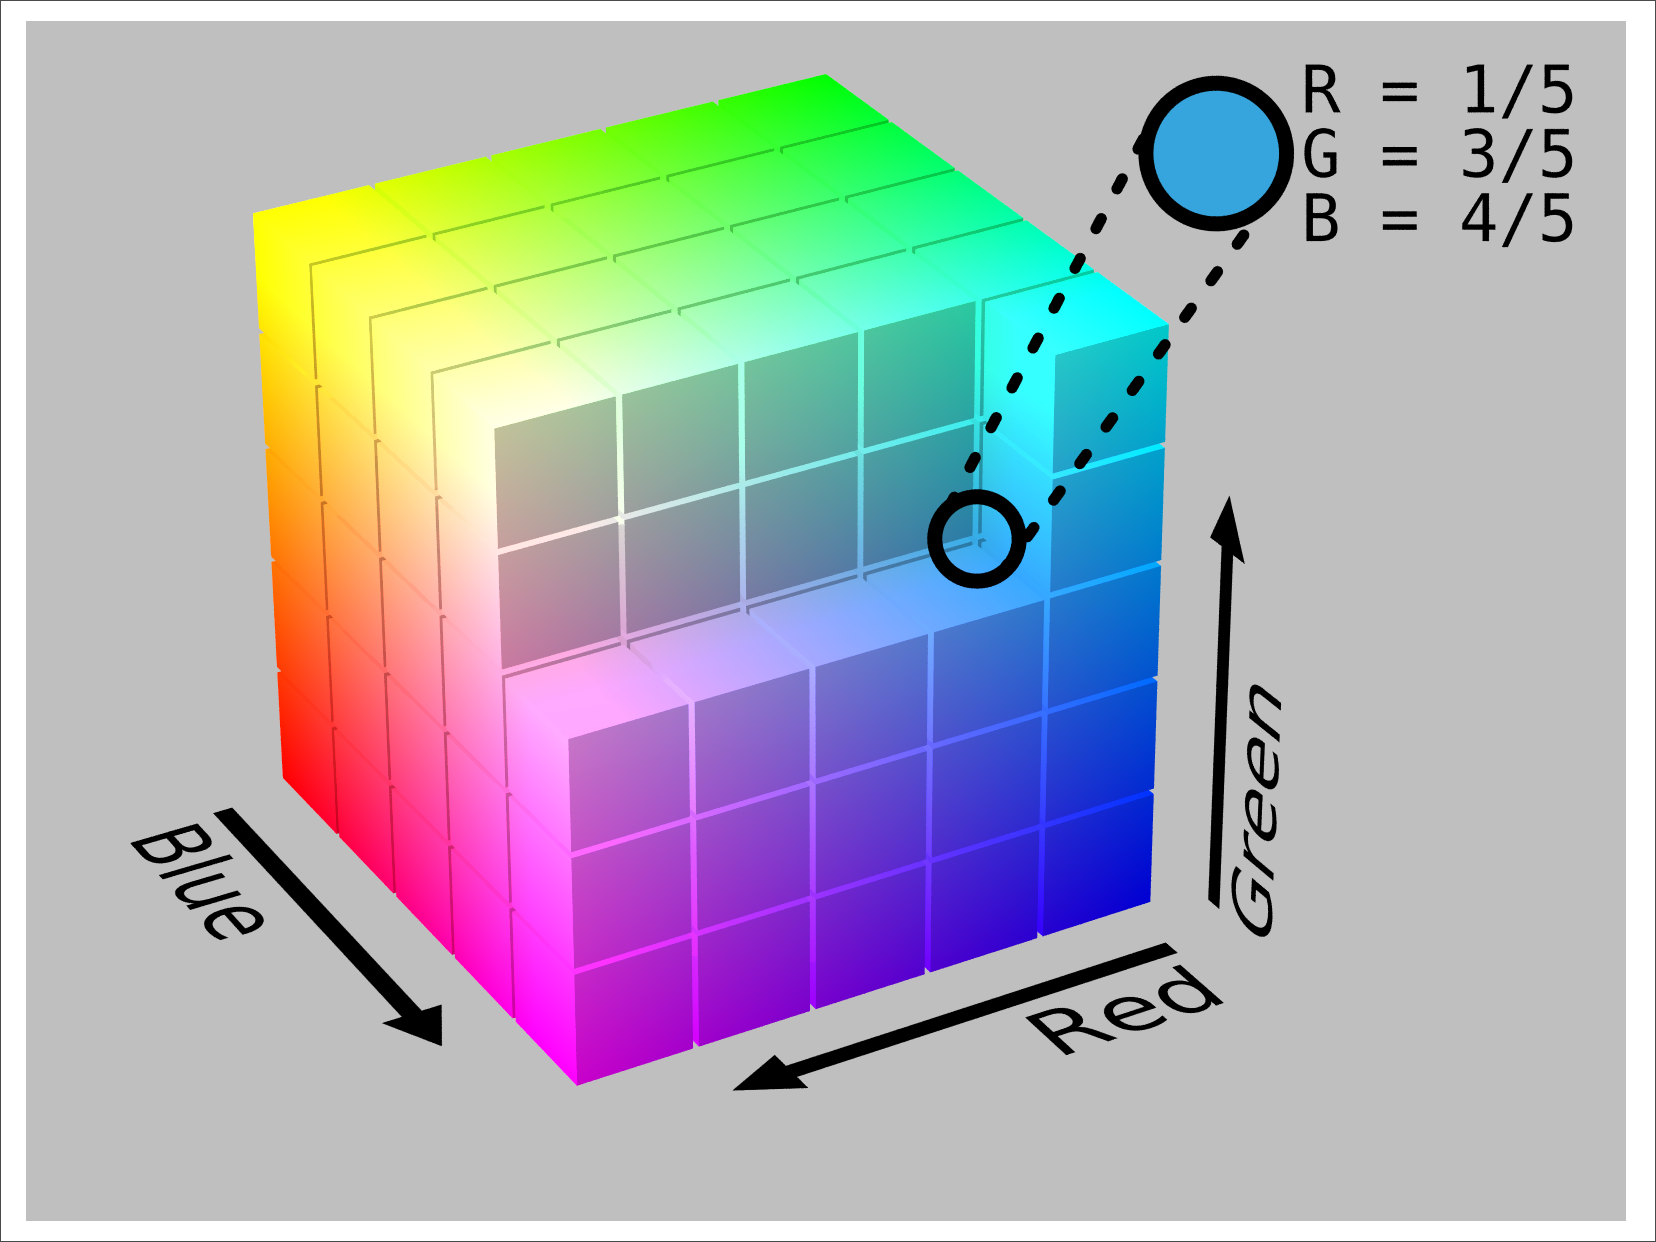
\includegraphics[width=0.9\textwidth]{rgb-cube}
\caption{ปริภูมิสี (Color Space) ในแบบลูกบาศก์ของพิกัดสีอาร์จีบี~\cite{RGBspace}}
%(ที่มา: http://wcm-birding.blogspot.com/2016/, 2560)
\label{fig:2-1}
\end{figure}

\begin{figure}[!ht]
\centering
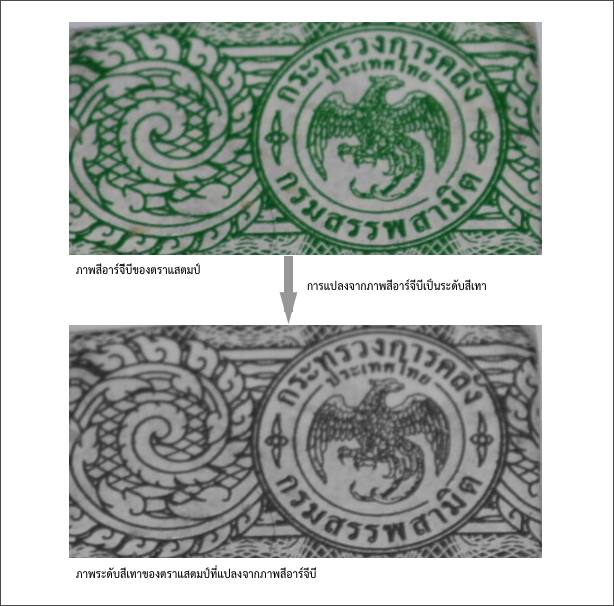
\includegraphics[width=0.9\textwidth]{rgb2gray-example}
\caption{ภาพระดับสีเทาที่ได้จากการแปลงจากภาพสีอาร์จีบี}
%(ที่มา: บริษัท เจ.เอฟ.แอดวาน.เมด.จำกัด, 2560)
\label{fig:rgb2gray}
\end{figure}

\subsection{ภาพระดับสีเทา}
ข้อมูลแสงในแต่ละพิกเซลของภาพระดับสีเทาเป็นค่าความเข้มแสง (light intensity) ระดับความเข้มแสงแต่ละระดับแสดงผลออกมาเป็นสีเทาหนึ่งสี  โดยระดับความเข้มสูงสุดจะเป็นสีขาว และระดับความเข้ม 0 จะเป็นสีดำ  จำนวนระดับสีเทา  (grayscale) ขึ้นอยู่กับจำนวนบิตของการบอกระดับ เช่นภาพระดับสีเทาขนาด 8 บิต บอกระดับสีเทาได้ 256 ระดับจาก 0 ถึง 255 

เราสามารถคำนวณระดับสีเทาของสีอาร์จีบีได้โดยการหาค่าเฉลี่ยแบบมีน้ำหนัก (weighted average) ของระดับแสงของแม่สี RGB เนื่องจากโดยธรรมชาติแล้วการมองเห็นแสงแต่ละสีไม่เท่ากัน   ค่าน้ำหนักที่เป็นที่นิยมในการคำนวณเพื่อแปลงสีอาร์จีบีเป็นระดับสีเทาเป็นไปตามสมการที่~\ref{eq:rgb2grey}  

\begin{equation}
Grey = 0.299R + 0.587G + 0.114 B \label{eq:rgb2grey}
\end{equation}
เมื่อ $R$, $G$ และ $B$ เป็นระดับแสงสีแดง สีเขียว และสีน้ำเงินตามลำดับ 
รูปที่~\ref{fig:rgb2gray} แสดงภาพสีเทาที่ได้จากการแปลงภาพสีอาร์จีบี


\subsection{ภาพขาวดำ (Binary Image) และการแปลงภาพระดับสีเทาเป็นภาพขาวดำ}
ข้อมูลแสงในแต่ละพิกเซลของภาพขาวดำ (Binary image) มีเพียง 2 สถานะ ซึ่งสามารถแทนด้วยข้อมูล 1 บิต โดย 0 แทนสีขาว และ    1 แทนสีดำ  เราอาจพูดได้ว่าภาพขาวดำก็คือภาพระดับสีเทาที่บอกระดับแสงด้วยข้อมูล 1 บิต 

กระบวนการในการแปลงภาพระดับสีเทาเป็นภาพขาวดำ เป็นการกระทำพื้นฐาน (basic operation) ของการประมวลผลภาพ  โดยมีหลายวิธีการแปลงภาพระดับสีเทาเป็นภาพขาวดำ เช่น วิธีการหาขอบ (edge detection) แต่ไม่ว่าจะเป็นวิธีการแปลงใดก็ตาม หลักการของการแปลงภาพระดับสีเทาเป็นภาพขาวดำคือการเปรียบเทียบกับค่าเทรซโฮลด์ตามสมการที่~(\ref{eq:background-thresholding})

\begin{equation}
B(x,y) = \left\{ \begin{array}{ll}
1, \mbox{ถ้าเงื่อนของการแปลงเป็นจริง เช่น}\ I(x,y) >= I_{th}\\
0, \mbox{กรณีอื่น ๆ}
\end{array}\right. \label{eq:background-thresholding}
\end{equation}
เมื่อ $0$ แทนส่วนสีดำ, $1$ แทนส่วนสีขาว, $B(x,y)$ และ $I(x,y)$ เป็นค่าข้อมูลสีของพิกเซล $(x,y)$ ในภาพขาวดำและภาพระดับสีเทา ตามลำดับ และในกรณีตัวอย่างนี้ $I_{th}$ เป็นค่าระดับเทรซโฮลที่ใช้


เงื่อนไขในการแปลจุดพิกเซลของภาพให้เป็นสีขาว ($1$)  หรือสีดำ ($0$)  นั้นขึ้นอยู่กับจุดประสงค์ของการแปลงภาพ ยกตัวอย่างวิธีการแปลงเป็นภาพขาวดำง่ายที่สุดคือ การใช้ระดับความเข้มแสงเป็นเทรซโฮลด์ในการแยกเพื่อแยกภาพออกเป็น 2 ลักษณะพื้นที่  ในบางกรณี เงื่อนไขการแบ่งจะขึ้นอยู่กับข้อมูลสีของพื้นที่รอบจุดพิกเซลที่สนใจ

%ที่นำมาใช้ ในกรณีของการลบภาพพื้นหลัง  มีจุดประสงค์ของการแยกระหว่างภาพพื้นหลัง (background) ออกจากภาพส่วนหน้า (foreground) ซึ่งเป็นส่วนที่สนใจในการนำไปประมวลผล การลบพื้นหลังใช้หลักการของการหาฮิสโตแกรม (histogram)  ของภาพซึ่งเป็นการนับการกระจายความเข้มแสงภายในภาพว่าอยู่ที่ส่วนใด ตามธรรมชาติของภาพแล้ว พื้นหลังของภาพจะมีความเข้มที่จับกลุ่มกันอยู่ทางด้านใดด้าหนึ่ง กล่าวคือสำหรับภาพที่พื้นหลังค่อนไปทางมืด ความเข้มของภาพพื้นหลังจะรวมกลุ่มอยู่ทางด้านซ้ายของฮิสโตแกรม แต่กลับกันภาพพื้นหลังมีความสว่าง เช่นภาพถ่ายของหิมะที่ปกคลุมพื้นที่ จะมีความเข้มของภาพพื้นหลังที่จับกลุ่มกันอยู่ทางด้านขวาของฮิสโตแกรม ดังแสดงในรูปที่~\ref{fig:bw}

จะเห็นว่าวิธีการเทรซโฮลเป็นวิธีการแบ่งพื้นที่ในภาพตามช่วงของระดับความเข้มแสง ซึ่งหลักการนี้สามารถใช้ได้กับข้อมูลระดับความเข้มแสงได้ทุกชนิด เช่น เราสามารถแบ่งภาพเป็น 2  ส่วนตามระดับสีเขียว หรือสีแดง หรือสีน้ำเงิน สีใดสีหนึ่งเพียงสีเดียวก็ได้ ด้วยหลักการเดียวกัน เราสามารถการแบ่งพื้นที่ของภาพออกเป็นมากกว่า 2 ส่วนก็ได้ เช่น เราอาจต้องการแบ่งพื้นที่ในภาพเป็น 4 ส่วน ซึ่งแทนด้วยข้อมูล 2 บิต ซึ่งในกรณีนี้จะต้องมีค่าเทรซโฮล 2 ตัวเพื่อการแบ่งระดับความเข้มแสงเป็น 4 ส่วน เรียกวิธีการแบ่งระดับที่ผลลัพธ์มีมากกว่า 2 ส่วนว่า การแบ่งหลายส่วน (multiband threshold)


\section{การหาขอบของวัตถุ (Edge Detection)}
การหาขอบ (Edge Dectection) ภายในภาพ เป็นการกระทำพื้นฐาน (basic operation) ของการประมวลผลภาพ  ที่มีการนำไปใช้จำนวนมาก เนื่องจากขอบภาพเป็นสารสนเทศพื้นฐานที่สำคัญ กล่าวคือขอบภายในภาพเป็นสารสนเทศพื้นฐานในการแบ่งส่วน การบอกรูปร่าง ซึ่งจะนำไปสู่การตรวจจับหาส่วนของภาพที่สนใจ (interested region) ทำให้เกิดตัดข้อมูลภาพส่วนที่ไม่เกี่ยวข้องออกไป เช่น ในโครงงานศึกษาวิจัยนี้ ต้องการตัดเอาเฉพาะส่วนที่เป็นตราของแสตมป์เท่านั้น


การหาขอบเป็นการแปลงภาพระดับสีเทาเป็นภาพขาวดำอย่างหนึ่ง โดยต้องการให้ส่วนที่เป็นสีขาวแทนขอบของวัตถุที่อยู่ในภาพ เทคนิคของการหาขอบมีหลายวิธี  แต่สามารถแบ่งออกได้เป็น 2 กลุ่ม หลักคือ วิธีการเกรย์เดียน (Gradient method) และ วิธีการลาปาซ (Laplacian method) สำหรับการหากรอบด้วยวิธีเกรย์เดียน  จะใช้การหาจุดต่ำสุดและจุดสูงสุดในรูปของอนุพันธ์อันดับหนึ่งของภาพ  วิธีการหาขอบในกลุ่มนี้ได้แก่ Sobel, Roberts, Prewitt และ Canny เป็นต้น ส่วนวิธีลาปาซ  จะหาขอบโดยใช้อนุพันธ์อันดับ 2 โดยใช้จุดที่ค่าจุดศูนย์ (Zero-crossing) ของอนุพันธ์อันดับ 2 ในภาพ ตัวอย่างวิธีการหาขอบในกลุ่มนี้ได้แก่ Laplacian of Gussian และ Marrs-Hildreth สำหรับโครงงานศึกษาวิจัยนี้ได้เลือกใช้วิธี Canny ในการหาขอบภาพ เพราะจากเอกลักษณ์ของภาพ  คือ  มีรูปร่างที่เด่นชัด ทำให้ไม่จำเป็นที่การหาขอบภาพจะต้องละเอียดมาก  แต่จะต้องสามารถหาขอบภาพได้ผลลัพธ์ในระดับ  ดังนั้นจึงเลือกใช้วิธี Canny 

การหาขอบด้วยวิธี Canny ใช้วิธีเกรย์เดียน ซึ่งมีขั้นตอนดังนี้
\begin{enumerate}
\item กรองภาพด้วยการกรอง Gaussian
\item หาเวคเตอร์เกรย์เดียนของพิกเซล ($x,y$) ตามสมการที่~(\ref{eq:gradient})
\begin{equation}
\nabla f(x,y) = \left[
\begin{array}{l}
G_x(x,y)\\
G_y(x,y)
\end{array}
\right] = \left[
\begin{array}{l}
\frac{\partial }{\partial x}f(x,y)\\
\frac{\partial }{\partial y}f(x,y)
\end{array}
\right]\label{eq:gradient}
\end{equation}
เมื่อ $\nabla f(x,y)$ เป็นเวคเตอร์เกรย์เดียนที่พิกเซล $(x,y)$ ของอนุพันธ์ย่อยของความเข้มแสง $f(x,y)$  ในแกน $x$ และแกน $y$ โดย $G_x$ และ $G_y$ เป็นอนุย่อยของ $f(x,y)$ ในแนวแกน $x$ และ $y$ ตามลำดับ
\item เปรียบเทียบขนาดของเกรย์เดียน $\nabla f(x,y)$  ตามสมการที่~(\ref{eq:gradient-abs}) กับค่าเทรซโฮลด์ $T$  เพื่อตัดสินว่าพิกเซล $(x,y)$ เป็นส่วนหนึ่งของขอบหรือไม่ตามสมการที่~(\ref{eq:edge}) และหาว่าขอบที่จุดพิกเซล $(x,y)$ อยู่ในทิศทาง $0$, $45$, $90$, หรือ $135$ องศา จากการหามุม $\theta (x,y)$ ตามสมการ~\ref{eq:gradient-theta}
\begin{eqnarray}
G(x,y) &=& |\nabla f(x,y)| \sqrt{G_x(x,y)^2 + G_y(x,y)^2}\label{eq:gradient-abs}\\
\theta (x,y) &=& \tan^{-1}\frac{G_y}{G_x}\label{eq:gradient-theta}\\
E(x,y) &=&\left\{ \begin{array}{ll}
1 & \mbox{if}\ G(x,y)  > T\\
0 & \mbox{otherwise}
\end{array}
\right.\label{eq:edge}
\end{eqnarray}
\item ขจัดขอบปลอมโดยวิธี non-maximum suppression
\item ใช้เทคนิคของ 2 เทรซโฮลด์ (Double threshold) ในการกำจัดขอบปลอม
\item ต่อขอบ (edge tracking) ด้วยเทคนิคฮิสเตอรีซีส (hysteresis)
\end{enumerate}

\begin{figure}[!ht]
\centering

\includegraphics[width=0.9\textwidth]{edge-example}
\caption{ตัวอย่างของผลการหาขอบด้วยวิธี Canny ของภาพระดับสีเทาในรูปที่~\ref{fig:rgb2gray}}
%(ที่มา: บริษัท เจ.เอฟ.แอดวาน.เมด.จำกัด, 2560)
\label{fig:edege-example}
\end{figure}

รูปที่~\ref{fig:edege-example} แสดงภาพผลลัพธ์ของการหาขอบด้วยวิธี Canny ของภาพแสตมป์ในรูปที่~\ref{fig:rgb2gray} 

\section{การแปลงฮัฟวงกลม (Circle Hough Transform)}
การแปลงฮัฟ (Hough transform) เป็นเทคนิคสำหรับการตรวจจับส่วนของเส้นตรง (line) หรือเส้นโค้ง (curve) ภายในภาพ แม้ว่าโดยหลักการแล้ววิธีการแปลงฮัฟจะสามารถใช้กับภาพอินพุทที่เป็นภาพระดับสีเทาก็ได้ แต่เราจะใช้การแปลงฮัฟกับภาพขาวดำ หรือภาพที่เป็นผลจากการหาขอบ เพราะวิธีการแปลงฮัฟต้องใช้การคำนวณและหน่วยความจำสูง

\begin{figure}[!ht]
\centering
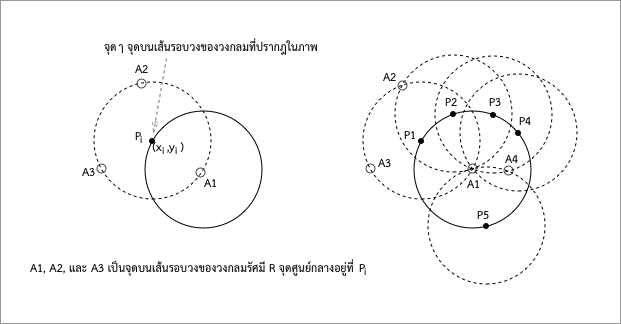
\includegraphics[width=0.9\textwidth]{Hough-transform-concept}
\caption{แนวคิดของการแปลงฮัฟวงกลม (Circle Hough Transform)}
%(ที่มา: บริษัท เจ.เอฟ.แอดวาน.เมด.จำกัด, 2560)
\label{fig:hough-concept}
\end{figure}
การแปลงฮัฟวงกลม เป็นกรณีพิเศษของการแปลงฮัฟ โดยมีหลักการว่า ถ้าเราสร้างวงกลมรอบจุดที่อยู่บนเส้นรอบวงของวงกลม วงกลมเหล่านี้จะไปตัดกันที่จุดศูนย์กลางของวงกลม ตามที่แสดงในรูปที่~\ref{fig:hough-concept} ด้านขวาจะเห็นว่า  วงกลมรัศมี $R$ 5 วงที่มีจุดศูนย์กลางที่จุด $P_1$, $P_2$, $P_3$, $P_4$, และ $P_5$ ซึ่งต่างเป็นเป็นจุดบนเส้นรอบวงของวงกลมรัศมี $R$ ในภาพขาวดำ จะตัดกันที่จุด $A_1$ ซึ่งเป็นจุดศูนย์กลางของวงกลมในภาพขาวดำ 

การแปลงฮัฟวงกลมใช้หลักการดังกล่าว ในการค้นหาจุดศูนย์กลางของวงกลมรัศมี $R$ ดังนี้
สำหรับจุด $P_i = (x_i, y_i)$ ใด ๆ ที่เป็นจุดที่อยู่บนขอบภายในภาพ ในขั้นตอนแรกของการแปลงฮัฟวงกลมจะเป็นการสร้างวงกลมรอบจุด $P_i$ ทุกจุดตามสมการที่~(\ref{eq:circle})
\begin{equation}
(x - x_i)^2 + (y-y_i)^2 = R^2\label{eq:circle}
\end{equation}
โดยที่ $(x_i, y_i)$ เป็นจุดที่อยู่บนขอบ (ค่าความเข้มแสงของจุดเท่ากับ $1$) ในภาพขาวดำที่ได้จากการหาขอบ และ $(x,y)$ เป็นจุดบนวงกลมรัศมี $R$ ที่มีจุดศูนย์กลางงอยู่ที่ $(x_i,y_i)$ ตามที่แสดงในรูปที่~\ref{fig:hough-concept} ด้านซ้ายมือ

ในกระบวนสร้างวงกลมตามสมการ~(\ref{eq:circle}) นั้น จะมีการนับความถี่ของการที่จุด $(x, y)$ ใด ๆ  ไปอยู่บนเส้นรอบวงของวงกลมที่สร้างตามสมการที่~(\ref{eq:circle}) ยกตัวอย่างเช่น ในรูปที่~\ref{fig:hough-concept} ด้านขวามือมีการสร้างวงกลม 5 วง จุด $A_3$ เป็นจุดที่อยู่บนเส้นรอบวงของวงกลมเหล่านี้ 1 ครั้ง ในขณะที่จุด $A_2$ และ $A_4$ เป็นจุดที่อยู่บนเส้นรอบวงของวงกลม 2 ครั้ง และจุด $A_1$ อยู่บนเส้นรอบวงของวงกลม 5 วง  ผลลัพธ์ของการกระทำดังกล่าวนี้จะเป็นเมตริกความถี่ของการเกิด โดยที่เมตริกนี้มีค่าที่ตำแหน่ง $(x,y)$ เป็นจำนวนครั้งที่วงกลมตามสมการที่~(\ref{eq:circle}) ไปตัดกันที่จุด $(x,y)$ 

ขั้นตอนต่อมาของการแปลงฮัฟวงกลม เป็นการเลือกจากเมตริกซ์ของจำนวนครั้งที่วงกลมไปตัดกันที่จุด $(x,y)$ ว่าจะจุดใดบ้างที่เป็นจุดศูนย์กลางของวงกลมรัศมี $R$ โดยเกณฑ์ในการเลือกจะมาจาก 2 วิธี คือ (1) การเรียงลำดับ และ (2) การใช้เทรซโฮลด์ หรือทั้ง 2 อย่างรวมกัน วิธีการเรียงลำดับจะใช้ได้กับภาพที่รู้ว่ามีจำนวนของวงกลมรัศมี R อยู่เท่าไร ถ้าทราบจำนวนดังกล่าว สมมุติว่าเป็น $n$ ตัวแล้ว เราสามารถเลือกจุดที่เป็นจุดศูนย์กลางของวงกลม จากการเรียงลำดับแล้วเลือก $n$ ตัวแรก แต่ในกรณีที่ไม่ทราบว่ามีวงกลมอยู่กี่วง การใช้เทรซโอลจะเหมาะสมกว่า กล่าวคือ ถ้าจำนวนความถี่น้อยกว่าค่าเทรซโฮลด์แสดงว่าไม่มีวงกลม แต่ถ้ามากกว่าแสดงว่ามีวงกลม หรือส่วนของวงกลมรัศมี R อยู่

\begin{figure}[!ht]
\centering
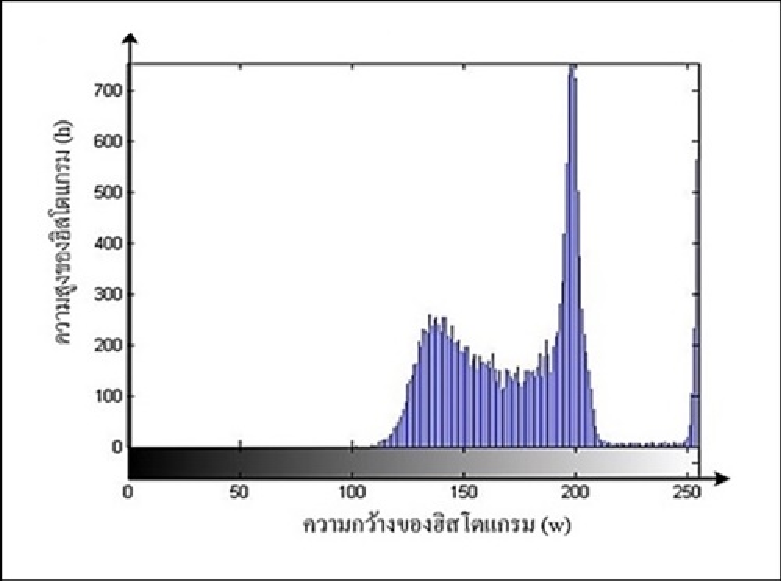
\includegraphics[width=0.9\textwidth]{histogram-example}
\caption{ตัวอย่างฮิสโตแกรมของระดับสีเทาของภาพในรูปที่~\ref{fig:rgb2gray}}
%(ที่มา: บริษัท เจ.เอฟ.แอดวาน.เมด.จำกัด, 2560)
\label{fig:histogram}
\end{figure}

\section{ฮิสโตแกรมของภาพ (Image Histogram)}
ฮิสโตแกรมเป็นการนับจำนวนความถี่ของการเกิดขึ้นของค่าของตัวแปรสุ่มจากกลุ่มข้อมูลจำนวนหนึ่ง ในกรณีของฮิสโตแกรมของภาพขนาด $c\times r$ พิกเซล ตัวแปรสุ่มคือระดับสี หรือระดับความเข้มแสง ซึ่งอาจจะเป็นระดับสีเทา หรือระดับสีใดสีหนึ่งของอาร์จีบี หรือระดับ H ในระบบสี HSV เป็นต้น ส่วนข้อมูลที่ใช้ในการนับคือระดับสีจากทุกพิกเซลของภาพ

ในกระบวนการนับจะต้องมีการสร้างกล่อง (Bin) ที่จะนับข้อมุลลงไป หนึ่งกล่องจะเป็นหนึ่งช่วงของตัวแปรสุ่ม โดยทั่วไปแล้วช่วงทั้งหมดของตัวแปรสุ่มจะแบ่งถูกแบ่งเป็น $n$ กล่องเท่ากัน ในกรณีของภาพ ตัวแปรสุ่มคือระดับความเข้มแสงซึ่งเป็นเลขจำนวนเต็มในช่วง 0 ถึง 255  (ในกรณีของระดับสีขนาด 8 บิท) ดังนั้นการแบ่งที่มีขนาดกล่องเล็กที่สุดคือ การใช้หนึ่งระดับสีเป็นหนึ่งกล่องรวมทั้งหมด  256 กล่อง

ในการสร้างฮิสโตแกรมของภาพ พิกเซลจะถูกตรวจสอบทีละพิกเซลว่ามีค่าระดับสีอยู่ในกล่องใด ผลลัพธ์การพล็อตฮิสโตแกรมจะเป็นการกระจายของโอกาสการเกิด รูปที่~\ref{fig:histogram} แสดงผลของฮสโตแกรมของภาพระดับสีเทาในรูปที่~\ref{fig:rgb2gray}

%
% การสร้าง accumulator cell ในกรณีวงกลมจะเป็น A(i, j) 3 มิติซึ่งพารามิเตอร์จะประกอบด้วย Cx, Cy และ r สำหรับวิธีการคำนวณหาพิกัด x, y ที่อยู่บนวงกลมหรือส่วนโค้งอันเดียวกันจะใช้วิธีการเช่นเดียวกันกับกรณีของเส้นตรง ในทำนองเดียวกันการหาส่วนโค้งและวงกลมด้วย Hough Circle Transform จะใช้สมการ
%
% \begin{displaymath}
%(x-c_x)^{2}+ (y-c_y)^{2}=r^{2}
%\end{displaymath}



\chapter{วิธีการตรวจสอบตราของแสตมป์ที่นำเสนอ}
\label{ch:proposed}
ในบทนี้จะเป็นการอธิบายวิธีการตรวจสอบตราของแสตมป์สุราโดยอัตโนมัติที่นำเสนอในโครงงานวิจัยนี้  โดยวิธีการที่นำเสนอใช้วิธีการทางการประมวลผลภาพ  ในหัวข้อ 3.1 จะเป็นการอธิบายโครงสร้างของระบบเพื่อใช้ในการถ่ายภาพ หัวข้อ 3.2 อธิบายแนวคิดและภาพรวมของวิธีที่นำเสนอ ซึ่งประกอบไปด้วย 2 ขั้นตอนหลักคือการตัดภาพรูปนกวายุภักษ์ และการนำภาพรูปนกวายุภักษ์ ไปตรวจสอบว่าเป็นแสตมป์แท้หรือปลอม ซึ่งจะอธิบายแต่ละส่วนนี้ในหัวข้อ 3.3 และ 3.4 ตามลำดับ
\section{โครงสร้างระบบเพื่อใช้ในการถ่ายภาพของแสตมป์}
ระบบตรวจสอบแสตมป์อัตโนมัติที่นำเสนอใช้วิธีการทางการประมวลผลภาพ ดังนั้นการถ่ายภาพจึงมีความสำคัญกับวิธีที่จะนำเสนอ โดยสำหรับในโครงงานวิจัยนี้ ได้กำหนดระบบการถ่ายภาพไว้ดังรูปที่~\ref{fig:hardware}

\begin{figure}[!ht]
\centering
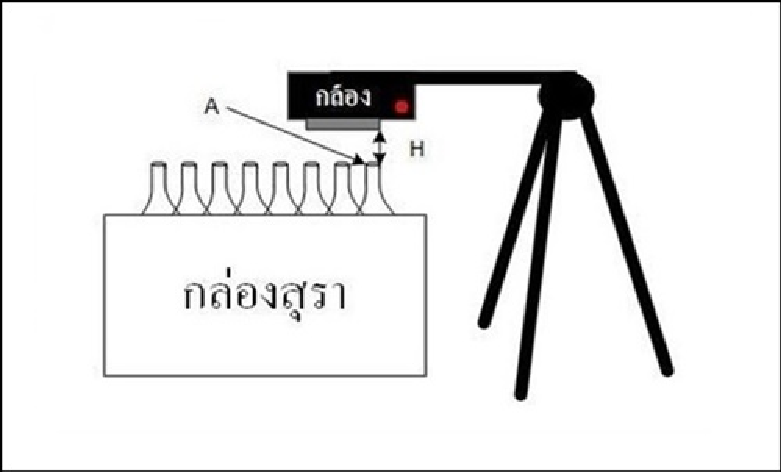
\includegraphics[width=0.9\textwidth]{capture-hardware}
\caption{โครงสร้างทางฮาร์ดแวร์ของระบบการคัดแยกตราของแสตมป์}
\label{fig:hardware}
\end{figure}

เนื่องจากแสตมป์เครื่องดื่มที่มีแอลกอฮอร์จะถูกกำหนดไว้ให้ติดไว้ที่บริเวณฝาผิดของขวด จึงได้กำหนดวิธีการถ่ายภาพไว้ให้เป็นการถ่ายจากด้านบน ด้วยกล้องถ่ายภาพสี ในพื้นที่ที่มีแสงเพียงพอ  ด้วยความสูงจากบริเวณแสตมป์ที่เหมาะสม การถ่ายภาพจะต้องให้ได้ภาพของตรานกวายุภักษ์ ที่อยู่ในแสตมป์ ดังตัวอย่างในรูปที่~\ref{fig:stamp-real} และ~\ref{fig:stamp-fake}  สำหรับกรณีแสตมป์จริงและแสตมป์ปลอมตามลำดับ

\begin{figure}[!ht]
\centering

\includegraphics[width=0.9\textwidth]{sample-stamp-real}
\vspace{2em}
\caption{ตัวอย่างรูปของแสตมป์จริงบริเวณตรานกวายุภักษ์ ที่ได้จากการถ่ายภาพ}
\label{fig:stamp-real}
\end{figure}

\begin{figure}[!ht]
\centering

\includegraphics[width=0.9\textwidth]{sample-stamp-fake}
\vspace{2em}
\caption{ตัวอย่างรูปของแสตมป์ปลอมบริเวณตรานกวายุภักษ์ ที่ได้จากการถ่ายภาพ}
\label{fig:stamp-fake}
\end{figure}

\section{แนวคิดของวิธีการตรวจสอบที่นำเสนอ}
จากการพิจารณารูปแสตมป์ตัวอย่างที่ถ่ายมาจำนวนหนึ่ง พบว่าลักษณะเด่นที่แตกต่างกันระหว่างแสตมป์จริงและแสตมป์ปลอมจะเกิดขึ้นบริเวณตรานกวายุภักษ์ โดยลักษณะที่เด่นที่สุดของความแตกต่างคือความเข้มของสีบริเวณตรานกวายุภักษ์  ดังแสดงในรูปที่~\ref{fig:stamp-real}  ซึ่งเป็นตัวอย่างรูปของแสตมป์จริง และ รูปที่~\ref{fig:stamp-fake}  ซึ่งเป็นตัวอย่างรูปของแสตมป์ปลอม จากข้อสังเกตดังกล่าวโครงงานวิจัยนี้จึงได้นำเสนอแนวคิดในการตรวจสอบแสตมป์ดังนี้

ในขั้นแรกของวิธีการคือ การตัดเอาเฉพาะส่วนของบริเวณตรานกวายุภักษ์ ออกมา ซึ่งเนื่องจากบริเวณตรานกวายุภักษ์ จะถูกล้อมรอบไว้ด้วยวงกลม โครงงานวิจัยนี้จึงมีแนวคิดในการนำเอาวิธีการทางการแปลงแบบวงกลมฮัฟ (Circle Hough Transform)  มาใช้ในการตัดเอาบริเวณตรานกวายุภักษ์ออกมา โดยจากการทดลองหลายครั้ง ทำให้ขนาดรัศมีวงกลมของตรานกวายุภักษ์ที่อยู่ในแสตมป์สุราว่าอยู่ในช่วงใด  เราจึงสามารถใช้วิธีการแปลงฮัฟวงกลมในการค้นหาวงกลมที่มีรัศมีอยู่ในช่วงดังกล่าวได้ โดยการเลือกเพียงวงกลมเดียวมา เพราะในภาพแสตมป์ที่ถ่ายมาจะมีตรานกวายุภักษ์เพียงตราเดียว รูปที่~\ref{fig:sample-hough} แสดงรูปตัวอย่างของผลของการใช้การแปลงฮัฟวงกลมในการค้นหาตรานกวายุภักษ์  และรูปที่~\ref{fig:sample-bird-cut} แสดงภาพที่ตัดเฉพาะส่วนที่เป็นนกวายุภักษ์ออกมาโดยการเลือกเอาเฉพาะภาพที่อยู่ภายในวงของวงกลมที่ได้จากการแปลงฮัฟวงกลม


\begin{figure}[!ht]
\centering

\includegraphics[width=0.9\textwidth]{sample-hough}
\vspace{2em}
\caption{ตัวอย่างผลของการใช้การแปลงฮัฟวงกลมแสดงด้วยเส้นสีแดงเพื่อค้นหาตรานกวายุภักษ์}
\label{fig:sample-hough}
\end{figure}

\begin{figure}[!ht]
\centering

\includegraphics[width=0.9\textwidth]{sample-bird-cut}
\vspace{2em}
\caption{รูปตัวอย่างของตรานกวายุภักษ์ที่ตัดจากภาพของแสตมป์โดยการตัดเอาเฉพาะส่วนที่อยู่ในวงกลมที่ได้จากการแปลงฮัฟวงกลม}
\label{fig:bird-cut}
\end{figure}


%\begin{figure}[!ht]
%\centering
%\includegraphics[width=0.9\textwidth]{355.jpg}
%\vspace{2em}
%\caption{ฮิสโตแกรมของรูปนกวายุภักษ์จากแสตมป์ปลอม}
%\label{fig:355}
%\end{figure}

\begin{figure}[!]
\centering
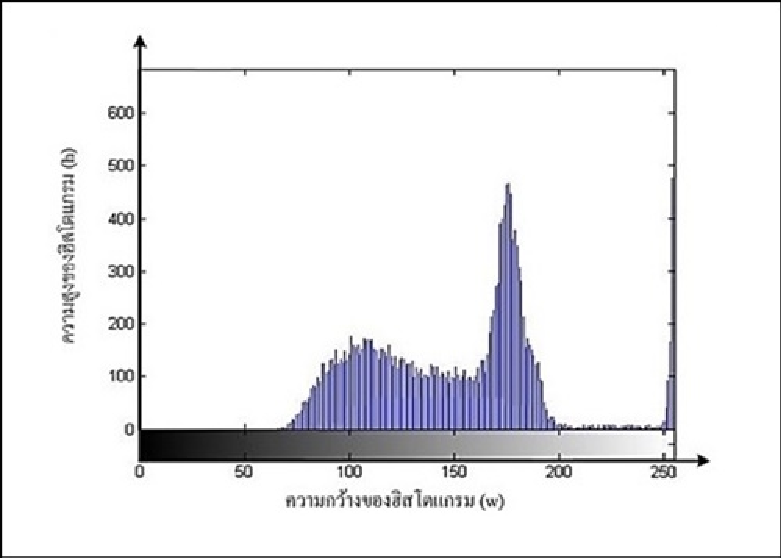
\includegraphics[width=0.81\textwidth]{histogram-real}
\vspace{2em}
\caption{ฮิสโตแกรมของรูปนกวายุภักษ์ที่ตัดมาจากแสตมป์จริง}
\label{fig:histogram-real}
\end{figure}
\begin{figure}[!]
\centering
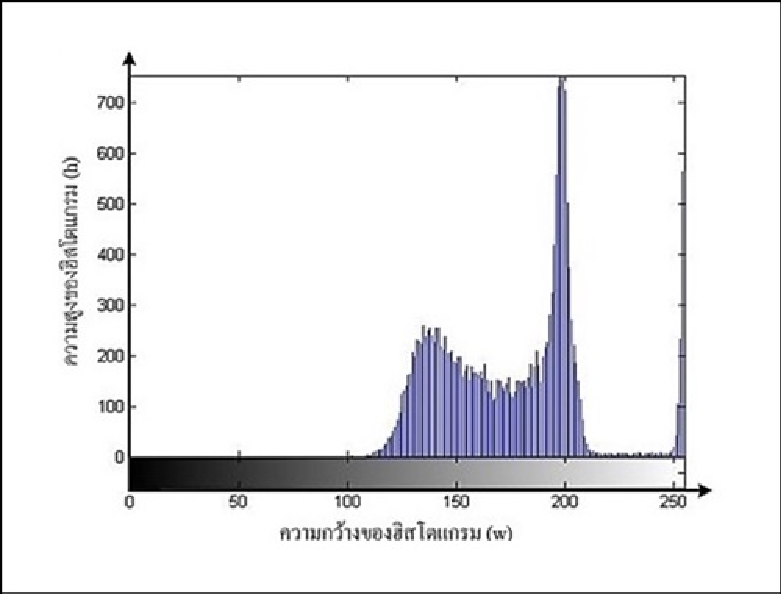
\includegraphics[width=0.81\textwidth]{histogram-fake}
\vspace{2em}
\caption{ฮิสโตแกรมของรูปนกวายุภักษ์ที่ตัดมาจากแสตมป์ปลอม}
\label{fig:histogram-fake}
\end{figure}

เมื่อสังเกตตรานกวายุภักษ์ ที่ตัดออกมาจากแสตมป์จริงและแสตมป์ปลอม จะพบว่าตรานกวายุภักษ์ ของแสตมป์จริงจะมีความเข้มมากกว่า และมีรายละเอียดมากกว่า เช่น บริเล็ปของนกในตราของจริงจะมีความชัดเจนมากกว่า คำถามของเราคือจะใช้วิธีการทางการประมวลผลภาพอะไรสำหรับการตรวจสอบความแตกต่างดังกล่าว  แนวคิดที่นำมาใช้ในโครงงานวิจัยนี้คือ ลองพิจารณาจากใช้วิธีที่ง่ายก่อน  ถ้าไม่ได้จึงพิจารณาใช้วิธีที่ยากซับซ้อนขึ้น

เนื่องจากความแตกต่างที่ชัดเจนคือความเข้มสี ดังนั้นจึงมีความเป็นไปได้ที่ฮิสโตแกรม (histogram) ของภาพตรานกวายุภักษ์จริงและภาพตรานกวายุภักษ์ปลอม จะบอกความแตกต่างได้  เนื่องจากสีที่ใช้พิมพ์แสตมป์เป็นสีเขียว จึงตัดเอาเฉพาะส่วนของสีเขียวไปสร้างฮิสโตแกรมดังแสดงในรูปที่~\ref{fig:histogram-real} และ~\ref{fig:histogram-fake}  สำหรับตรานกวายุภักษ์จริงและปลอมตามลำดับ จากการเปรียบเทียบคุณลักษณะเด่นของฮิสโตแกรม ของภาพส่วนสีเขียวของตรานกวายุภักษ์ของแสตมป์จริงและของแสตมป์ปลอม  พบว่าลักษณะของการกระจายของอิสโตแกรมคล้ายคลึงกัน กล่าวคือจะมีพื้นที่ของการกระจายของความเข้มสีเขียวอย่างต่อเนื่องกัน แต่มีลักษณะเด่นของฮิสโตแกรม 2 ประการที่แตกต่างกันคือ
\begin{enumerate}
\item ความกว้างของฮิสโตแกรมในส่วนที่ต่อเนื่องกัน ซึ่งพบว่าความกว้างของฮิสโตแกรมของตรานกวายุภักษ์ของแสตมป์จริงจะมากกว่า ของตรานกวายุภักษ์ของแสตมป์ปลอม สำหรับในโครงงานวิจัยนี้เราจะใช้สัญลักษณ์ $w$ แทนความกว้างของอิสโตแกรมดังกล่าวนี้
\item ความสูงที่สูงที่สุดของฮิสโตแกรมในส่วนที่ต่อเนื่องกัน ซึ่งพบว่าความสูงของอิสโตแกรมของตรา
นกวายุภักษ์ จากแสตมป์จริงจะมากกว่า ของตรานกวายุภักษ์ จากแสตมป์ปลอม สำหรับในโครงงานวิจัยนี้เราจะใช้สัญลักษณ์ $h$ แทนความสูงของอิสโตแกรมดังกล่าวนี้
\end{enumerate}

ด้วยคุณลักษณะของฮิสโตแกรมที่แตกต่างกัน 2 ข้อดังกล่าว เราสามารถนำไปใช้เป็นลักษณะเด่นในการคัดแยกว่าแสตมป์เป็นของจริงหรือปลอมได้ วิธีการคัดแยกที่นำมาใช้ในโครงงานศึกษาวิจัยนี้ เป็นวิธีการนำเอาลักษณะเด่นทั้งสองคือ ความกว้างของฮิสโตแกรม ($w$) และ ความสูงของฮิสโตแกรม ($h$) ไปพล็อตเป็นคู่พิกัด $(w, h)$ บนระนาบโดย $w$ เป็นแกน $x$ และ $h$ เป็นแกน $y$ แล้วใช้เส้นตรงบนระนาบดังกล่าวเป็นเส้นแบ่งกลุ่มของจริงกับของปลอม

จากแนวคิดของการแก้ปัญหาวิจัยดังกล่าว เราจะได้ภาพรวมของขั้นตอนการตรวจสอบแสตมป์ที่นำเสนอในโครงงานศึกษาวิจัยนี้ตามบล็อกไดอะแกรม (block diagram) ดังรูปที่~\ref{fig:block-diagram} โดยรายละเอียดของขั้นตอนการตัดเอาเฉพาะตรานกวายุภักษ์และการคัดแยกจะอธิบายไว้ในหัวข้อ~\ref{sec:bird-cut-method}~และ~\ref{sec:classification} ตามลำดับ

\begin{figure}[!ht]
\centering
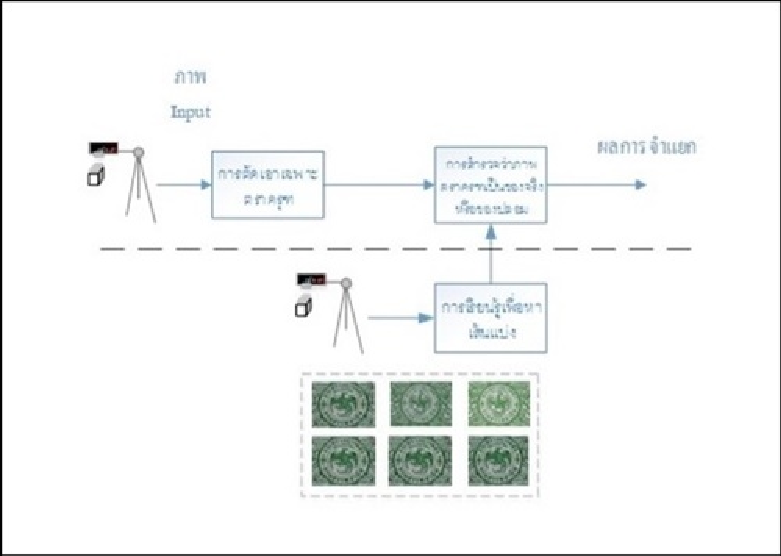
\includegraphics[width=0.9\textwidth]{block-diagram}
\vspace{2em}
\caption{บล็อกไดอะแกรมของวิธีการตรวจสอบแสตมป์อัตโนมัติ}
\label{fig:block-diagram}
\end{figure}


\section{วิธีการตัดเอาเฉพาะภาพตรานกวายุภักษ์}
\label{sec:bird-cut-method}
ตามที่ได้กล่าวไว้ในแนวคิดของการแก้ปัญหาแล้วว่าโครงงานวิจัยนี้ได้นำวิธีการแปลงแบบฮัฟ มาใช้เป็นเครื่องมือในการค้นหาวงกลมที่ล้อมรอบตรานกวายุภักษ์ที่อยู่ในแสตมป์ หัวข้อนี้อธิบายขั้นตอนการตัดเอาภาพตรานกวายุภักษ์ ดังกล่าวดังนี้

\begin{figure}[!ht]
\centering
\vspace{2em}

\includegraphics[width=0.9\textwidth]{input-image}
\vspace{2em}
\caption{ภาพของแสตมป์ที่ต้องการตรวจสอบ นำเข้าในโปรแกรมเพื่อการตัดเอาส่วนของตรานกวายุภักษ์}
\label{fig:input-image}
\end{figure}

\begin{figure}[!ht]
\centering
\vspace{2em}
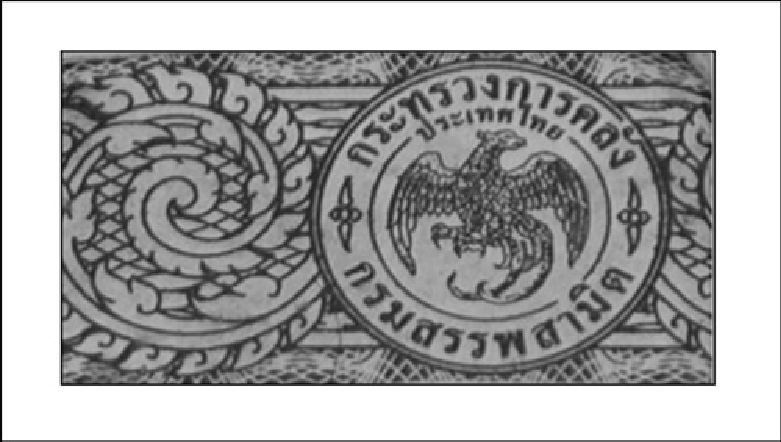
\includegraphics[width=0.9\textwidth]{grey-image}
\vspace{2em}
\caption{ภาพระดับสีเทาของภาพแสตมป์ในรูปที่~\ref{fig:input-image}}
\label{fig:grey}
\end{figure}

%\begin{itemize}

\textbf{ขั้นตอนที่ 1:} นำเข้าภาพแสตมป์ รูปที่~\ref{fig:input-image} แสดงภาพตัวอย่างของภาพแสตมป์ที่นำเข้าสู่กระบวนการ สังเกตว่าภาพอินพุทนี้มีการตัดเอาเฉพาะส่วนที่มีตราแสตมป์เท่านั้น ในโครงงานศึกษาวิจัยนี้เราจะสมมุติว่ามีระบบตัดภาพนี้ให้แล้ว

\textbf{ขั้นตอนที่ 2:} แปลงภาพจากขั้นตอนที่ 1 เป็นภาพระดับเทา รูปที่~\ref{fig:grey} แสดงผลของขั้นตอนนี้เมื่อใช้กับภาพตัวอย่างในรูปที่~\ref{fig:input-image}

\textbf{ขั้นตอนที่ 3:} แปลงภาพระดับเทาเป็นภาพขาวดำ รูปที่~\ref{fig:bw} แสดงผลของขั้นตอนนี้เมื่อใช้กับภาพระดับสีเทานรูปที่~\ref{fig:bw}

\textbf{ขั้นตอนที่ 4:} ใช้วิธีการหาเส้นขอบด้วยวิธี canny เพื่อการหาขอบ  โดยอินพุทเป็นภาพขาวดำจากขั้นตอนที่ 3 เพราะต้องการลดจำนวนจุดขาวของภาพลงไป รูปที่~\ref{fig:edge} เป็นผลของการหาขอบของภาพในรูปที่~\ref{fig:bw} 

\begin{figure}[!]
\centering
\vspace{2em}

\includegraphics[width=0.9\textwidth]{bw-image}
\vspace{2em}
\caption{ภาพขาวดำที่ได้จากการแปลงภาพระดับสีเทาของแสตมป์จากรูปที่~\ref{fig:grey}}
\label{fig:bw}
\end{figure}


\begin{figure}[!]
\centering
\vspace{2em}

\includegraphics[width=0.9\textwidth]{edge-image}
\vspace{2em}
\caption{ภาพที่ได้จากการหาเส้นขอบด้วยวิธี canny ของภาพตัวอย่างดังรูปที่~\ref{fig:bw}}
\label{fig:edge}
\end{figure}


\begin{figure}[!]
\centering
\vspace{2em}

\includegraphics[width=0.9\textwidth]{hough-result}
\vspace{2em}
\caption{ตัวอย่างผลลัพธ์ของการค้นหาวงกลมของภาพตัวอย่างในรูปที่~\ref{fig:input-image} ด้วยการใช้การแปลงฮัฟวงกลม}
\label{fig:hough-result}
\end{figure}


\begin{figure}[!]
\centering
\vspace{2em}

\includegraphics[width=0.9\textwidth]{bird-cut-image}
\vspace{2em}
\caption{ตัวอย่างผลของการตัดภาพอินพุทเพื่อเอาเฉพาะส่วนของภายในวงกลมที่ได้จากขั้นตอนที่ 6}
\label{fig:bird-cut-sample}
\end{figure}



\textbf{ขั้นตอนที่ 5:} ใช้การแปลงแบบฮัฟวงกลม (Circle Hough Transform) เพื่อสร้าง  Hough Space  ของวงกลมที่มีรัศมีในช่วงที่ครอบคลุม โดยใช้ขนาดของรัศมีวงนอกสุดของกรอบวงกลมที่ล้อมรอบตรานกวายุภักษ์เป็นขอบเขตสูงสุด

\textbf{ขั้นตอนที่ 6:} เลือกวงกลมจาก Hough Space ในขั้นตอนที่ 5 ที่มีความถี่ของการเกิดมากที่สุด ผลที่ได้ในขั้นนี้จะอยู่ในรูปของตำแหน่งจุดศูนย์กลางและรัศมี รูปที่~\ref{fig:hough-result} แสดงผลของวงกลมที่ได้จากภาพของแสตมป์ตัวอย่างดังรูปที่~\ref{fig:input-image}

\textbf{ขั้นตอนที่ 7:} ตัดเอาเฉพาะส่วนของภาพอินพุทที่อยู่ภายในวงกลมที่ได้ในขั้นตอนที่ 6 รูปที่~\ref{fig:bird-cut-sample} แสดงภาพของการตัดสำหรับกรณีภาพตัวอย่างตามรูปที่~\ref{fig:input-image}
%\end{itemize}



%\begin{figure}[!ht]
%\centering
%\vspace{2em}
%\includegraphics[width=0.9\textwidth]{3-13}
%\vspace{2em}
%\caption{ภาพต้นฉบับเพื่อหาระยะความสูงของผู้ใช้บริการ และ กระบวนการประมวลผลภาพทำการคำนวณหาระยะความสูง แล้วส่งคำสั่งให้ชุดบอร์ดมอเตอร์ควบคุมระบบชุดรับภาพเอกซเรย์}
%\label{fig:3-13}
%\end{figure}

\section{วิธีการแยกแยะตรานกวายุภักษ์}
\label{sec:classification}
ตามที่ได้กล่าวไว้ในแนวคิดของการแก้ปัญหา ในโครงงานศึกษาวิจัยนี้  จะใช้คุณสมบัติเด่นของฮิสโตแกรมของภาพตรานกวายุภักษ์ ที่ได้จากการตัดด้วยวิธีที่นำเสนอตามหัวข้อที่~\ref{sec:bird-cut-method} เพื่อการตรวจสอบว่าแสตปม์นั้นเป็นของจริงหรือปลอม จากแนวคิดที่นำเสนอพบว่าคุณลักษณะ 2 ตัวของฮิสโตแกรมดังแสดงในรูปที่~\ref{fig:feature-def} ที่สามารถใช้ในการแยกแยะตราวายุภักษ์ของแสตมป์จริงกับของแสตมป์ปลอมออกจากกันคือ
\begin{enumerate}
\item ความสูงของฮิสโตแกรมของภาพตรานกวายุภักษ์ แทนด้วย $h$ เป็นค่าความถี่ที่ปรับให้อยู่ระหว่าง 0 ถึง 1 ที่มีค่าสูงสุด
\item ความกว้างของฮิสโตแกรมของภาพตรานกวายุภักษ์ แทนด้วย $w$ เป็นค่าความกว้างของฮิสโตแกรมทีมีความถี่มากกว่า 20/
\end{enumerate}

\begin{figure}[!ht]
\centering
\vspace{2em}
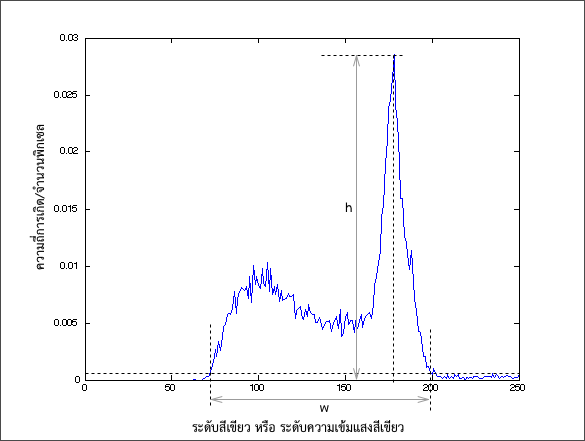
\includegraphics[width=0.9\textwidth]{historgram-norm}
\vspace{2em}
\caption{นิยามของค่า $w$ และ $h$  ที่ใช้เป็นลักษณะเด่นในการแยกแยะตรานกวายุภักษ์}
\label{fig:feature-def}
\end{figure}

วิธีการแยกแยะที่นำมาใช้ เป็นวิธีการใช้เส้นเบ่งแบบเส้นตรง (linear classification line) ของจุดพิกัด $(w,h)$ โดยจุดพิกัดที่ได้จากตราวายุภักษ์ของแสตมป์จริงจะอยู่ข้างล่างของเส้นแบ่ง เพราะฮิสโตแกรมของมันจะมีค่า $h$  (แกน $y$) ที่ต่ำของปลอม ในขณะที่ $w$ (แกน $x$) ของตราวายุภักษณ์ของจริงจะมีค่ามากกว่าของตราวายุภักษ์ปลอม  เส้นแบ่งดังกล่าวจะใช้วิธีการเรียนรู้ซี่งอธิบายในหัวข้อ~\ref{sec:training} 

วิธีการแยกแยะตราวายุภักษณ์ที่นำมีขั้นตอนดังนี้

\textbf{ขั้นตอนที่ 1:} นำเข้าภาพตรานกวายุภักษ์ ที่ได้จากขั้นตอนการตัดภาพตรานกวายุภักษ์ดังตัวอย่างในรูปที่~\ref{fig:bird-cut-sample} ไปหาฮิสโตแกรมของระดับสีเขียว ได้ผลลัพธ์ดังตัวอย่างในรูปที่~\ref{fig:histogram-example}

\textbf{ขั้นตอนที่ 2:} ปรับความถี่ของฮิสโตแกรมให้เป็นค่าระหว่าง 0 ถึง 1 โดยการหารด้วยจำนวนจุดของภาพ

\textbf{ขั้นตอนที่  3:} ตัดฮิสโตแกรมให้เหลือเฉพาะส่วนของ Bin  จาก 21 ถึง 250 เพื่อให้ใต้เฉพาะส่วนของฮิสโตแกรมที่ต่อเนื่อง 

\textbf{ขั้นตอนที่ 4:} หาความสูง $h$ ได้โดยการหาค่าที่มากที่สุดของกราฟอิสโตแกรมจากขั้นตอนที่ 3

\textbf{ขั้นตอนที่ 5:} หาความกว้าง $w$ ตามนิยามตามรูปที่~\ref{fig:feature-def}

\textbf{ขั้นตอนที่ 6:} ถ้า $(w,h)$ อยู่ใต้เส้นแบ่งแสดงว่าเป็นภาพตรานกวายุภักษ์อินพุทเป็นของแสตมป์จริง ถ้าไม่เช่นนั้นแสดงว่าเป็นของแสตมป์ปลอม

%\begin{figure}[!ht]
%\centering
%\vspace{2em}
%\includegraphics[width=0.9\textwidth]{3-13}
%\vspace{2em}
%\caption{ภาพต้นฉบับเพื่อหาระยะความสูงของผู้ใช้บริการ และ กระบวนการประมวลผลภาพทำการคำนวณหาระยะความสูง แล้วส่งคำสั่งให้ชุดบอร์ดมอเตอร์ควบคุมระบบชุดรับภาพเอกซเรย์}
%\label{fig:3-13}
%\end{figure}


\begin{figure}[!ht]
\centering
\vspace{2em}
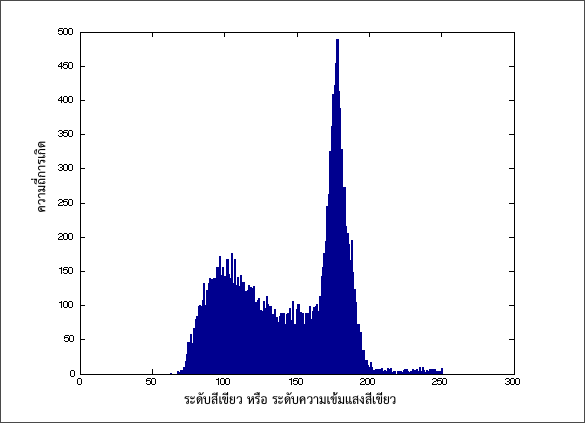
\includegraphics[width=0.9\textwidth]{histogram-example-stamp}
\vspace{2em}
\caption{ตัวอย่างอิสโตแกรมของภาพระดับสีเขียวของตรานกวายุภักษ์จากรูปที่~\ref{fig:bird-cut-sample}}
\label{fig:histogram-example}
\end{figure}

\begin{figure}[!hb]
\centering
\vspace{2em}
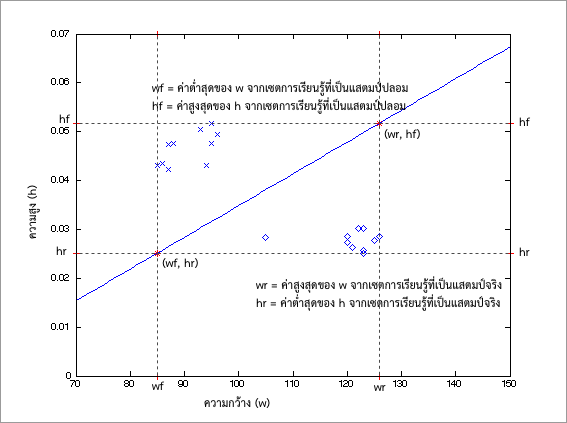
\includegraphics[width=0.81\textwidth]{training-method}
\vspace{2em}
\caption{เส้นตรงสำหรับการแยกแยะที่ได้จากการเรียนรู้ด้วยภาพแสตมป์จริงและแสตมป์ปลอมอย่างละ 5 ภาพ ($n=5$)}
\label{fig:training-result}
\end{figure}

\section{การเรียนรู้เพื่อหาเส้นแบ่งการคัดแยก}
\label{sec:training}
เส้นตรงที่ใช้ในการตัดสินว่าภาพตรานกวายุภักษ์เป็นของแสตมป์จริงหรือปลอมหาได้จากการเรียนรู้โดยมีขั้นตอนดังต่อไปนี้

\begin{enumerate}
\item เลือกเซตของภาพที่ใช้ในการเรียนรู้  โดยใช้ภาพจากแสตมป์จริงและแสตมป์ปลอมจำนวน $n$ ภาพเท่ากัน   ให้ $r_1, r_2,\ldots r_n$ เป็นภาพตรานกวายุภักษ์ที่ตัดจากแสตมป์จริงจำนวน $n$ ภาพ และให้ $f_1, f_2,\ldots , f_n$ เป็นภาพตรานกวายุภักษ์ที่ตัดจากแสตมป์ปลอมจำนวน $n$ ภาพ
\item ใช้วิธีการตัดตราวายุภักษ์ที่เสนอในหัวข้อ~\ref{sec:bird-cut-method}  ในการตัดภาพวายุภักษณ์ของภาพที่ใช้ในการเรียนรู้ทั้งหมด
\item ใช้วิธีการหาค่า $w$ และ $h$ ของตราวายุภักษณ์ที่ตัดมาทุกอัน โดยให้ $w_r(i)$ และ $h_r(i)$ เป็นค่า $w$ และ $h$ ของภาพในการเรียนรู้ที่เป็นแสตมป์จริงลำดับที่ $i$ และให้ $w_f(i)$ และ $h_f(i)$ เป็นค่า $w$ และ $h$ ของภาพในการเรียนรู้ที่เป็นแสตมป์ปลอมลำดับที่ $i$, $i = 1, 2,\ldots n$
\item หาเส้นตรงที่เป็นเส้นแบ่งกลุ่มของ $(w_r(i), h_r(i))$ ออกจากกลุ่มของ $(w_f(i), h_f(i))$ 
\begin{itemize}
\item เลือกมุมซ้ายล่างของกลุ่ม $(w_{min}, h_{min})$ และจุดมุมขวาของกลุ่ม $(w_{max}, h_{max})$ โดยที่
\begin{itemize}
\item $w_{min}$ เป็นค่าน้อยที่สุดของ   $w_f$ 
\item $h_{min}$ เป็นค่าน้อยที่สุดของ $h_r$ 
\item $w_{max}$ เป็นค่าน้อยที่สุดของ   $w_r$ 
\item $h_{max}$ เป็นค่าน้อยที่สุดของ $h_f$ 
\end{itemize}
\item เลือกเส้นแบ่งเป็นเส้นตรงจากจุด $(w_{min},h_{min})$ ซึ่งเป็นจุดด้านมุมซ้ายล่างกับจุด $(w_{max}, h_{max})$ ซึ่งเป็นจุดมุมขวาบน
\end{itemize}
\end{enumerate}
 
 รูปที่~\ref{fig:training-result} แสดงตัวอย่างของผลการเรียนรู้ด้วย $n=10$




\chapter{การทดสอบและการวิจารณ์}
\label{ch:results}
วิธีการตรวจสอบแสตมป์ตามที่นำเสนอในบทที่ 3 ได้รับการทวนสอบ (verification) ด้วยการทดลองกับภาพแสตมป์จริงและแสตมป์ปลอมอย่างละ 20 ภาพ ในหัวข้อ 4.1 จะบอกถึงข้อมูลของกล้องและระบบคอมพิวเตอร์รวมทั้งโปรแกรมที่ใช้ในการทดสอบ หัวข้อ 4.2 จะบอกถึงผลที่ได้จากการทดสอบ และหัวข้อ 4.3 เป็นการวิจารณ์ผลการทดสอบที่ได้


\section{การเตรียมการในการทดสอบ}
 \subsection{ระบบฮาร์ดแวร์และซอฟท์แวร์ที่ใช้ในการทดสอบ} 
 \label{sec:setup}
ในการทดลองเพื่อทดสอบวิธีการที่นำเสนอ ระบบการถ่ายภาพแสตมป์แบบง่าย ตามที่นำเสนอในบทที่ 3 ได้ถูกสร้างขึ้น เพื่อการถ่ายภาพแสตมป์ที่ใช้ในการทดสอบ สำหรับกล้องที่ใช้ในการถ่ายภาพเป็นกล้องดิจิทัลซึ่งมีข้อมูลของกล้องตามที่แสดงในตารางที่~\ref{tab:camera}

\begin{table}[htb]
\caption{ข้อมูลกล้องที่ใช้ในการถ่ายภาพสแตมป์}
\label{tab:camera}
\begin{tabular}{ll}
\hline
รุ่นของกล้อง            &NIKON D5200\\
จำนวนจุดพิกเซล      &24.1 megapixels\\
เลนส์                    &18 -55 VR\\
ระยะโฟกัส             &Contrast Detect (sensor\\
ความเร็วชัตเตอร์      &30 sec-1/4000 sec\\
การซูม                  &35-55 mm\\
\hline
\end{tabular}
\end{table} 


วิธีการที่นำเสนอได้ถูกนำสร้างบนแพล็ตฟอร์ม Matlab โดยการเขียนเป็นโปรแกรมรันบนคอมพิวเตอร์ส่วนบุคคล

\subsection{ข้อมูลสำหรับการทดลอง}
ภาพของแสตมป์สำหรับการทดสอบได้จากการถ่ายภาพด้วยกล้องถ่ายภาพตามหัวข้อ~\ref{sec:setup} ในการทดสอบระบบจำเป็นต้องมีภาพแสตปม์ทั้งที่เป็นแสตมป์จริง และแสตมป์ปลอมจำนวน 2 เซต โดยทั้งหมดเป็นสแตมป์ที่ได้จากสรรพากรเขตพื้นที่จังหวัดอุบลราชธานี โดยมีรายละเอียดของแสตมป์ตัวอย่างตามตารางที่~\ref{tab:data}

\begin{table}[htb]
\caption{ข้อมูลแสตมป์ที่ใช้ในการทดลอง}
\label{tab:data}
\begin{tabular}{ll}
\hline 
ชนิดของแสตมป์       &เป็นแสตมป์สุราของสรรพากรเขตพื้นที่จังหวัดอุบลราชธานี\\
จำนวนแสตมป์ทั้งหมด          &50 แสตมป์\\
จำนวนแสตมป์จริง               & 25 แสตมป์\\
จำนวนแสตมป์ปลอม            &25 แสตมป์\\
\hline
\end{tabular}
\end{table} 

\subsection{การเรียนรู้เพื่อหาเส้นตรงที่ใช้เป็นเกณฑ์การตรวจสอบ}

ตามวิธีการที่นำเสนอในบทที่ 3 การตรวจสอบว่าแสตมป์เป็นของจริงหรือของปลอม จะต้องมีการเรียนรู้เพื่อสร้างเกณฑ์สำหรับการตรวจสอบ ซึ่งเป็นเส้นตรงบนระนาบ $w-h$ โดย 
               $w$ เป็นความกว้างของฮิสโตแกรมของภาพระดับสีเขียวของตรานกวายุภักษ์ในแสตมป์ และ
               $h$ เป็นความสูงที่สุดของอิสโตแกรมของภาพระดับสีเขียวของตรานกวายุภักษ์ในแสตมป์ 
              กระบวนการในการเรียนรู้เป็นไปตามที่อธิบายไว้ในหัวข้อ~\ref{sec:training}

สำหรับในการทดสอบนี้ ได้เลือกภาพแสตมป์จำนวน 10 ภาพเป็นสแสตมป์จริงและแสตมป์ปลอมอย่างไร 5 ภาพ เพื่อใช้เป็นเซตของภาพสำหรับการเรียนรู้ (training set) ผลการเรียนรู้เป็นไปตามที่แสดงในรูปที่~\ref{fig:training-result} ซึ่งเป็นสมการเส้นตรงตามสมการที่~\ref{eq:classification-line}

\begin{figure}[!ht]
\centering
\vspace{2em}
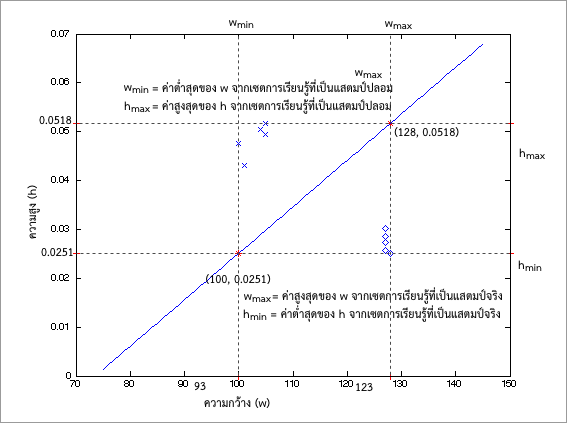
\includegraphics[width=0.9\textwidth]{training-result-n5}
\vspace{2em}
\caption{กราฟจากการพล็อตจุดพิกัด $(w,h)$ ที่ได้จากการเรียนรู้ด้วยเซตของภาพสำหรับการเรียนรู้}
\label{fig:training-result}
\end{figure}

\begin{eqnarray}
%\frac{h - h_{min}}{w - w_{min}} &=& \frac{h_{max} - h_{min}}{w_{max}-w_{min}} \nonumber\\
h &=& m*(w - w_{0}) + h_{0} \label{eq:classification-line}\\
m &=& \frac{h_{max} - h_{min}}{w_{max}-w_{min}} = 8.881\times 10^{-4}\nonumber\\
w_0 &=& w_{min} = 100\nonumber\\
h_0 &=& h_{min}  = 0.0251\nonumber\\\nonumber
\end{eqnarray}

 โดยที่  
 \begin{itemize}
 \item $w_{min}$ เป็นค่าต่ำสุดของ $w$ ที่ได้จากชุดข้อมูลสำหรับการเรียนรู้ กลุ่มแสตมป์ปลอม  
 \item[]จากการทดลองได้ $w_{min} = 100$
 \item $w_{max}$ เป็นค่าสูงสุดของ $w$ ที่ได้จากชุดข้อมูลสำหรับการเรียนรู้ กลุ่มแสตมป์จริง 

 \item[]จากการทดลองได้ $w_{max} = 128$
\item $h_{min}$ เป็นค่าต่ำสุดของ $h$ ที่ได้จากชุดข้อมูลสำหรับการเรียนรู้ กลุ่มแสตมป์จริง 

\item[]จากการทดลองได้ $h_{min} = 0.0251$ 
\item $h_{max}$ เป็นค่าสูงสุดของ $h$ ที่ได้จากชุดข้อมูลสำหรับการเรียนรู้ กลุ่มแสตมป์ปลอม 

\item[]จากการทดลองได้ $h_{max} = 0.0518$ 
\item $m$ เป็นความชันของเส้นแบ่ง จากการทดลองได้
\item $(w_0, h_0)$ เป็นจุด ๆ หนึ่งบนเส้นแบ่งในที่นี้เลือกใช้จุด $(w_{min}, h_{min})$
 \end{itemize}
 

           

\section{ผลการทดสอบและการวิจารณ์}
วิธีการที่นำเสนอมี 2 ขั้นตอนหลัก คือ (1) การตัดเอาเฉพาะตรานกวายุภักษ์ และ (2) การตรวจสอบว่านกวายุภักษณ์ที่ตัดมาเป็นของจริงหรือของปลอม ดังนั้นในการทดสอบจึงแบ่ง 2 ขั้นตอน 
โดยภาพที่ที่ใช้ในการทดสอบเป็นภาพที่ไม่อยู่ในเซตของการเรียนรู้ โดยเป็นภาพแสตมป์จริง 20 ภาพ และภาพแสตมป์ปลอม  20  ภาพ

\subsection{ผลการตัดรูปนกวายุภักษ์} 
 ในขั้นตอนแรกเป็นการทดสอบเพื่อพิจารณาผลการตัดเอาเฉพาะตรานกวายุภักษ์ รูปที่~\ref{fig:bird-cut-result-r}~และ~\ref{fig:bird-cut-result} แสดงผลการตัดสำหรับแสตมป์ที่เป็นแสตมป์จริง และแสตมป์ปลอมตามลำดับ

\begin{figure}[!ht]
\centering
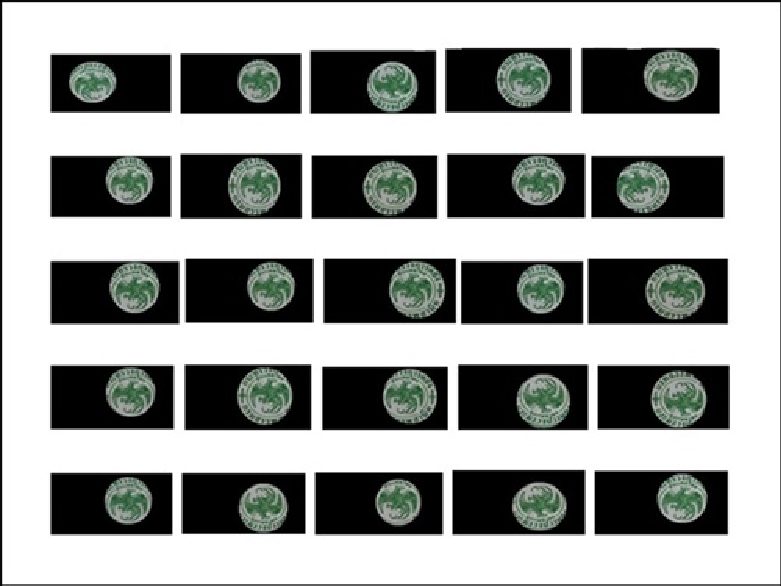
\includegraphics[width=0.9\textwidth]{bird-cut-result-r}
\caption{ภาพนกวายุภักษ์ที่ได้จากผลการตัดจากภาพแสตมป์จริงที่ใช้ในการทดสอบ}
\label{fig:bird-cut-result-r}
\end{figure}

\begin{figure}[!ht]
\centering
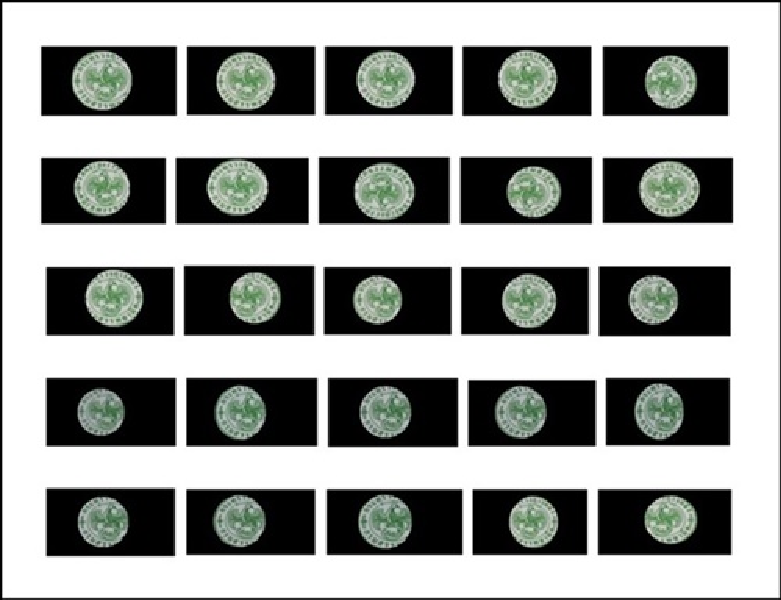
\includegraphics[width=0.9\textwidth]{bird-cut-result-f}
\caption{ภาพนกวายุภักษ์ที่ได้จากผลการตัดจากภาพแสตมป์ปลอมที่ใช้ในการทดสอบ}
\label{fig:bird-cut-result-f}
\end{figure}
 

จากรูปที่~\ref{fig:bird-cut-result-r}~และ~\ref{fig:bird-cut-result-f} การตัดเอาภาพของนกวายุภักษ์เพื่อไปใช้ในการตรวจสอบนั้น ไม่ได้ถูกต้องทั้งหมด ภาพการตัดที่ไม่ถูกต้องจะมีลักษณะที่มีบางส่วนภายในกรอบของรูปครุฑที่หายไป และอาจจะมีบางภาพที่มีส่วนอื่นเพิ่มขึ้นมา  ทั้งนี้เพราะตรานกวายุภักษ์ซี่งอยู่ในกรอบวงกลม ภายในภาพแสตมป์ที่ใช้ทดลอบนั้น ตัววงกลมล้อมรอบรูปครุฑจะไม่สมดุล  กล่าวคือจะมีลักษณะเป็นวงรี  ทำให้การตัดซึ่งเป็นการตัดด้วยวงกลมมีความคลาดเคลื่อนในบางส่วน เหตุผลที่ภาพเป็นวงรีนั้นมาจากขั้นตอนการถ่ายภาพ ซึ่งควบคุมให้ภาพเป็นวงกลมทั้งหมดได้ยาก

อย่างไรก็ตามผลการตัดที่คลาดเคลื่อนดังกล่าวนี้มีผลกระทบกับการแยกแยะไม่มาก เพราะลักษณะเด่นที่ใช้ในการวิเคราะเป็นคุณสมบัติของการกระจายของสีเขียวของส่วนที่เป็นตรานกวายุภักษ์ ซึ่งผลของการคลาดเคลื่อนจะเป็นผลต่อจุดพิกัดของ $(w, h)$ อยู่บ้างแต่มีไม่มากพอที่จะให้เกิดการย้ายกลุ่ม

\begin{figure}[!hb]
\centering
\vspace{2em}
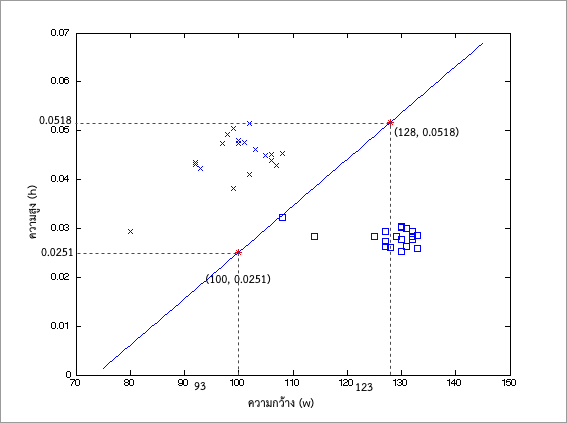
\includegraphics[width=0.9\textwidth]{testing-result}
\vspace{2em}
\caption{กราฟจากการพล็อตจุดพิกัด $(w,h)$ ที่หาได้จากภาพตรานกวายุภักษ์ที่ตัดมาจากภาพแสตมป์ที่ใช้ทดสอบ}
\label{fig:classification-result}
\end{figure}

\subsection{ผลการแยกแยะชนิดของแสตมป์} 

ภาพที่ได้จากการตัดรูปนกวายุภักษ์จะถูกนำไปตรวจสอบว่าเป็นภาพของแสตมป์จริงหรือของแสตมป์ปลอม โดยการนำข้อมูลสีเขียวของภาพที่ตัดได้ไปหาฮิสโตแกรม แล้วปรับให้ฮิสโตแกรมไปทำให้อยู่ในช่วงเดียวกันคือมีค่าระหว่าง 0 ถึง 1 เหมือนกัน ทั้งนี้เพราะภาพที่ตัดมาอาจมีขนาดภาพไม่เท่ากัน จากนั้นจึงหาค่า $w$ และ $h$ ของแต่ละภาพ นำค่า $w$ และ $h$ ที่ได้ไปเปรียบกับเส้นแบ่งที่ได้จากการเรียนรู้ ถ้าจุด $(w,h)$ อยู่เหนือเส้นแบ่งแสดงว่าเป็นภาพตรานกวายุภักษ์นั้นเป็นของแสตมป์ปลอม รูปที่~\ref{fig:classification-result} แสดงผลพล็อตจุด $(w,h)$ ของภาพทดสอบทั้งหมด โดยกากบาทเป็นจุดของภาพทดสอบที่เป็นแสตมป์ปลอม ส่วนเครื่องหมายรูปเพชรเป็นจุดของภาพทดสอบที่เป็นแสตมป์จริง 



ถ้าจุดเครื่องหมายกากบาทอยู่ใต้เส้นแบ่ง แสดงว่าเป็นการตัดสินผิดจากของปลอมเป็นของจริง ซึ่งไม่พบกรณีนี้เกิดขึ้นจากภาพตัวอย่างที่ใช้ทดสอบ
ถ้าจุดรูปเพชร อยู่เหนือเส้นแบ่ง แสดงว่าเป็นการตัดสินผิดจากของจริงเป็นของปลอม ซึ่งไม่พบกรณีนี้เกิดจากภาพตัวอย่างที่ใช้ทดสอบ
สรุปได้ว่าวิธีที่นำเสนอสามารถตรวจสอบแสตมป์ตัวอย่างจำนวน 40 แสตมป์ได้ทั้งหมด



จากผลการทดสอบพบว่าวิธีที่นำเสนอสามารถตรวจสอบแสตมป์ตัวอย่างที่ใช้ทดสอบทั้งหมด 40 แสตมป์ได้ทั้งหมด ซึ่งแสดงว่าวิธีที่นำเสนอมีโอกาสที่จะถูกนำไปใช้งานได้จริง อย่างไรก็ตามแม้ยังมีประเด็นที่ต้องให้ความสนใจดังต่อไปนี้
\begin{enumerate}
\item ตามวิธีที่นำเสนอนั้น การตัดรูปครุฑมีความสำคัญอย่างยิ่งเพราะเกณฑ์ในการตัดขึ้นอยู่กับฮิสโตแกรมของรูปครุฑเท่านั้น ถ้าตัดรูปครุฑผิดฮิสโตแกรมอาจจะมีคุณสมบัติที่แตกต่าง ทำให้ตัดสินผิด หรือในบางกรณีตัดสินใจไม่ได้เลย   แต่อย่างไรก็ตามแม้ว่าภาพที่ถ่ายมาวงกลมจะปรากฏเป็นวงรี ผลการตัดก็ยังถูกต้องในแง่ที่สามารถตัดเอาส่วนใหญ่ของรูปครุฑออกมาได้ทุกกรณีของภาพตัวอย่าง 
\item ปัญหาที่อาจจะเกิดได้กับการตัดตรานกวายุภักษ์คือ กรณีที่แสตมป์ที่ติดอยู่ที่ขวดมีความไม่สมบูรณ์ เช่น มีบางส่วนหายไป หรือแสตมป์มีการขาด ซึ่งจะเป็นปัญหาวิจัยในอนาคตเพื่อทำให้สามารถนำวิธีการที่นำเสนอไปใช้งานได้จริง
\item สำหรับขั้นตอนการหาจุดพิกัด (w, h) จากอิสโตแกรมของรูปครุฑ มีความเป็นไปได้ที่อาจจะเกิดปัญหาขึ้นเมื่อในการนำวิธีที่นำเสนอไปใช้งานจริง ในกรณีที่มีความไม่เท่ากันของแสงที่ใช้ ซึ่งอาจจะส่งผลต่อเส้นแบ่งที่ได้จากการเรียนรู้มาก่อน จึงเป็นอีกกรณีหนึ่งที่จะต้องทำการศึกษาเพื่อเพิ่มเติม
\item ประเด็นสุดท้ายคือวิธีการที่นำเสนอตั้งอยู่บนฐานของแสตมป์ปลอมเพียงกลุ่มเดียว ดังนั้นจึงเป็นไปไม่ได้ที่จะบอกว่าวิธีการที่นำเสนอนี้สามารถตรวจสอบแสตมป์ได้ทุกชนิด 
\end{enumerate}



 
 







          
           


\chapter{บทสรุป}
โครงงานศึกษาวิจัยนี้ได้นำเสนอวิธีการตรวจสอบแสตมป์สุราว่าเป็นแสตมป์ของจริงหรือของปลอม โดยแสตมป์สุราที่สนใจเป็นแสตมป์สุราที่นำเข้า หรือเรียกอีกอย่างว่าแสตมป์สุราต่างประเทศซึ่งเป็นสุราที่มีราคาสูง ทำให้มีการลักลอบนำเข้า แล้วนำมาติดตราแสตมป์ปลอมเพื่อหลีกเลี่ยงการเสียภาษีสรรพากร 
วิธีที่กรมสรรพสามิตในเขตพื้นที่ต่าง ๆ ใช้ในการตรวจสอบแสตมป์สุรานำเข้าคือ การใช้ผู้เชี่ยวชาญในการตรวจ ซึ่งมีจำนวนคนน้อย จึงทำให้ไม่สามารถตรวจสอบการลักลอบได้อย่างทั่วถึง ปริมาณการลักลอบก็สูงขึ้นเนื่องจากผู้ลักลอบทราบว่าเจ้าหน้าที่มีน้อยจึงกล้าเสี่ยง

โครงงานศึกษาวิจัยนี้ได้เสนอให้ใช้การประมวลผลภาพในการตรวจสอบความเป็นของแท้ของแสตมป์สุรา โดยภาพที่ใช้ในการทดสอบเป็นภาพของแสตมป์ที่ถ่ายจากด้านบนของขวดด้วยกล้องดิจิทัล วิธีที่นำเสนอเป็นวิธีที่ง่ายโดยใช้ฮัพวงกลมในการตัดเอาเฉพาะตรานกวายุภักษ์ออกมาก่อน แล้วนำไปหาคุณลักษณะเด่น ก่อนที่จะนำไปตัดสินว่าเป็นแสตมป์จริงหรือปลอม คุณลักษณะเด่นที่ใช้ในการแยกเป็นคุณลักษณะของฮิสโตแกรมของสีเขียวของภาพนกภายุภักษ์ที่ตัดมา โดยมี 2 ตัวคือ ความสูงที่มากที่สุดของฮิสโตแกรมเรียกว่า $h$ และความกว้างของฮิสโตแกรมเรียกว่า $w$ วิธีการแยกแยะใช้เส้นตรงในระนาบของ $(w,h)$ ที่ได้จากการเรียนรู้แบบง่ายจากเซตของภาพแสตมป์ทั้งของจริงและของปลอม

ผลการทดสอบกับแสตมป์ที่ได้มาจากกรมสรรพสามิตเขตพื้นที่ จังหวัดอุบลราชธานี จำนวน 40 แสตมป์ เป็นแสตมป์จริงและปลอมอย่างละ 20 แสตมป์พบว่าวิธีที่นำเสนอสามารถตรวจสอบได้อย่างถูกต้องทั้งหมด แต่มีแสตมป์จริงบางตัวที่มีคุณสมบัติใกล้เคียงกับแส้นแบ่างที่ได้จากการเรียนรู้

อย่างไรก็ตาม แม้ว่าผลการทดสอบจะมีอัตราการตรวจสอบถูกต้องที่สูงเป็นที่น่าพอใจ แต่การที่จะนำวิธีการเช่นนี้ไปใช้จริงอาจจะต้องพิจารณาประเด็นต่าง ๆ อีกหลายประเด็น ได้แก่  (1) การถ่ายภาพที่จะต้องอยู่ในระยะทีกำหนด และอาจจะต้องควบคุมแสงให้เพียงพอ (2) ปรับปรุงวิธีการแยกแยะเช่นการใช้ SVM (support vector machine) แทนเพราะวิธีที่นำเสนอใช้หลักการเดียวกัน (3) มีการเรียนรู้ด้วยภาพที่มากกว่า 5 ภาพที่ใช้อยู่ และ (4) วิธีที่นำเสนออาจใช้ได้ดีกับการปลอมแปลงที่สีของตรานกวายุภักษ์มีความแตกต่างกัน แต่ถ้ามีการปลอมแปลงแบบอื่นวิธีนี้อาจจะใช้ไม่ได้ อย่างไรก็ตามหลักการของการตัดเอามาเฉพาะตรานกวายุภักษ์ซึ่งเป็นส่วนที่มีรายละเอียดมาก จึงยากที่สุดที่จะปลอมแปลง เพีื่อมาวิเคราะห์ว่าเป็นของแท้หรือของปลอมเป็นแนวคิดที่มีโอกาสที่จะใช้ได้สูง




%%%%%%%%%%%%%%%%%%%%%%%%%%%%%%%%%%%%%%%%%%%%%%%%%%%%%%%%%%%%%%%
%%%%%%%%%%%%%%%%%%%% Bibliography %%%%%%%%%%%%%%%%%%%%%%%%%%%%%
%%%%%%%%%%%%%%%%%%%%%%%%%%%%%%%%%%%%%%%%%%%%%%%%%%%%%%%%%%%%%%%

%%%% Comment this in your report to show only references you have
%%%% cited. Otherwise, all the references below will be shown.
%\nocite{*}
%% Use the kmutt.bst for bibtex bibliography style 
%% You must have cpe.bib and string.bib in your current directory.
%% You may go to file .bbl to manually edit the bib items.
%\bibliographystyle{kmutt}
%\bibliography{bib/references}

%\bibliography{thesis-main-th.bbl}

%%%%%%%%%%%%%%%%%%%%%%%%%%%%%%%%%%%%%%%%%%%%%%%%%%%%%%%%%%%%%%%
%%%%%%%%%%%%%%%%%%%%%%%% Appendix %%%%%%%%%%%%%%%%%%%%%%%%%%%%%
%%%%%%%%%%%%%%%%%%%%%%%%%%%%%%%%%%%%%%%%%%%%%%%%%%%%%%%%%%%%%%%

%\appendix{หัวข้อภาคผนวกที่ 1}
\label{appendix1}
%\noindent{\large\bf This is a first appendix} \\
\clearpage

\begin{table}[!htb] 
\centering
\caption{ผู้ทดสอบที่ 1}
\label{tab:1}
\begin{tabular}{|c|c|c|c|}
\hline
\multicolumn{4}{|c|}{\textbf{ผู้ทดสอบที่ 1}}    \\ \hline
\textbf{ครั้งที่} & \textbf{ความสูง (ซม.)} & \textbf{เวลา(วินาที)} & \textbf{ค่าระยะห่างเส้นขอบ(ซม.)}  \\ \hline
1                 & 169.13                	& 18.9285               	& -13.02             	\\ \hline
2                 & 168.5                  	& 18.6329               	& -11.13     		   	\\ \hline
3                 & 169.13                	 & 18.9283               	& -11.13              	\\ \hline
4                 & 168.92                	 & 18.9285               	& -10.5          		 \\ \hline
5                 & 168.92                 	& 18.83                 	& -9.87      				\\ \hline
6                 & 168.92                 	& 18.83                 	& -7.35                     \\ \hline
7                 & 168.5                	 	& 18.63                 	& -7.14                      \\ \hline
8                 & 168.71                 	& 18.7314               	& -3.99                \\ \hline
9                 & 169.13                 	& 18.9285               	& -1.68                                       \\ \hline
10                & 169.13                	& 18.83                 	& -2.1                                           \\ \hline
\textbf{average}  & 168.90                 & 18.82                 & -7.79                                    \\ \hline
\end{tabular}
\end{table}

\begin{figure}[!ht]
\centering
\includegraphics[width=14cm]{AP1.jpg}
\caption{ภาพผลการทดลองผู้ทดสอบที่ 1}
\label{fig:AP1.jpg}
\end{figure}


\begin{table}[!hb] 
\centering
\caption{ผู้ทดสอบที่ 2}
\label{tab:2}
\begin{tabular}{|c|c|c|c|}
\hline
\multicolumn{4}{|c|}{\textbf{ผู้ทดสอบที่ 2}}    \\ \hline
\textbf{ครั้งที่} & \textbf{ความสูง (ซม.)} & \textbf{เวลา(วินาที)} & \textbf{ค่าระยะห่างเส้นขอบ(ซม.)}  \\ \hline
1       & 169.97 & 19.3227 & 0.84   \\ \hline
2       & 169.97 & 19.3227 & 0.42  \\ \hline
3       & 170.18 & 19.4212 & 1.26  \\ \hline
4       & 170.18 & 19.4212 & 2.31  \\ \hline
5       & 170.18 & 19.4212 & 0.42  \\ \hline
6       & 170.18 & 19.4212 & 1.05    \\ \hline
7       & 169.97 & 19.3227 & 1.89   \\ \hline
8       & 170.18 & 19.4212 & 2.52    \\ \hline
9       & 169.97 & 19.3227 & 0.84  \\ \hline
10      & 169.76 & 19.2241 & 1.26  \\ \hline
average & 170.05 & 19.36   & 1.28 \\ \hline
\end{tabular}
\end{table}

\begin{figure}[!ht]
\centering
\includegraphics[width=14cm]{AP2.jpg}
\caption{ภาพผลการทดลองผู้ทดสอบที่ 2 }
\label{fig:AP2.jpg}
\end{figure}


\begin{table}[!hb] 
\centering
\caption{ผู้ทดสอบที่ 3}
\label{tab:3}
\begin{tabular}{|c|c|c|c|}
\hline
\multicolumn{4}{|c|}{\textbf{ผู้ทดสอบที่ 3}}    \\ \hline
\textbf{ครั้งที่} & \textbf{ความสูง (ซม.)} & \textbf{เวลา(วินาที)} & \textbf{ค่าระยะห่างเส้นขอบ(ซม.)} \\ \hline
1       & 179.21 & 23.6588 & -4.83  \\ \hline
2       & 179.75 & 23.9513 & -4.83      \\ \hline
3       & 179    & 23.6502 & 0        \\ \hline
4       & 179.21 & 23.6588 & 0.63     \\ \hline
5       & 179.48 & 23.2324 & 0        \\ \hline
6       & 179.8  & 21.444  & -1.68   \\ \hline
7       & 179.8  & 21.444  & -0.42     \\ \hline
8       & 179.53 & 23.7251 & 0.21    \\ \hline
9       & 179.63 & 23.8559 & 2.1   \\ \hline
10      & 179.9  & 23.495  & -0.63    \\ \hline
average & 179.53 & 23.21   & -0.95   \\ \hline
\end{tabular}
\end{table}

\begin{figure}[!ht]
\centering
\includegraphics[width=14cm]{AP3.jpg}
\caption{ภาพผลการทดลองผู้ทดสอบที่ 3 }
\label{fig:AP3.jpg}
\end{figure}


\begin{table}[!hb] 
\centering
\caption{ผู้ทดสอบที่ 4}
\label{tab:4}
\begin{tabular}{|c|c|c|c|}
\hline
\multicolumn{4}{|c|}{\textbf{ผู้ทดสอบที่ 4}}    \\ \hline
\textbf{ครั้งที่} & \textbf{ความสูง (ซม.)} & \textbf{เวลา(วินาที)} & \textbf{ค่าระยะห่างเส้นขอบ(ซม.)} \\ \hline
1       & 165.9  & 17.4295 & -4.2 \\ \hline
2       & 165.32 & 17.6266 & -4    \\ \hline
3       & 165.16 & 17.0208 & -5.25     \\ \hline
4       & 165.85 & 17.9367 & -7.14    \\ \hline
5       & 165.74 & 17.8237 & -5.25    \\ \hline
6       & 165.74 & 17.8237 & -5.25  \\ \hline
7       & 165.74 & 17.8237 & -5.25      \\ \hline
8       & 165.95 & 17.9222 & -4.62   \\ \hline
9       & 165.79 & 17.3164 & -2.94     \\ \hline
10      & 165.16 & 17.0208 & -4.41     \\ \hline
average & 165.64 & 17.57   & -4.83    \\ \hline
\end{tabular}
\end{table}

\begin{figure}[!ht]
\centering
\includegraphics[width=14cm]{AP4.jpg}
\caption{ภาพผลการทดลองผู้ทดสอบที่ 4 }
\label{fig:AP4.jpg}
\end{figure}


\begin{table}[!hb] 
\centering
\caption{ผู้ทดสอบที่ 5}
\label{tab:5}
\begin{tabular}{|c|c|c|c|}
\hline
\multicolumn{4}{|c|}{\textbf{ผู้ทดสอบที่ 5}}    \\ \hline
\textbf{ครั้งที่} & \textbf{ความสูง (ซม.)} & \textbf{เวลา(วินาที)} & \textbf{ค่าระยะห่างเส้นขอบ(ซม.)}  \\ \hline
1       & 169.97 & 19.3227 & 0.84   \\ \hline
2       & 169.97 & 19.3227 & 0.42     \\ \hline
3       & 169.76 & 19.2241 & 0.21      \\ \hline
4       & 169.97 & 19.3227 & 1.26    \\ \hline
5       & 169.97 & 19.3227 & 2.31      \\ \hline
6       & 169.76 & 19.2241 & 2.1    \\ \hline
7       & 169.97 & 19.3227 & 1.05    \\ \hline
8       & 169.97 & 19.3227 & 0.84  \\ \hline
9       & 169.55 & 19.1256 & 1.26   \\ \hline
10      & 170.39 & 19.5198 & 2.73   \\ \hline
average & 169.93 & 19.30   & 1.30   \\ \hline
\end{tabular}
\end{table}

\begin{figure}[!ht]
\centering
\includegraphics[width=14cm]{AP5.jpg}
\caption{ภาพผลการทดลองผู้ทดสอบที่ 5 }
\label{fig:AP5.jpg}
\end{figure}


\begin{table}[!hb] 
\centering
\caption{ผู้ทดสอบที่ 6}
\label{tab:6}
\begin{tabular}{|c|c|c|c|}
\hline
\multicolumn{4}{|c|}{\textbf{ผู้ทดสอบที่ 6}}    \\ \hline
\textbf{ครั้งที่} & \textbf{ความสูง (ซม.)} & \textbf{เวลา(วินาที)} & \textbf{ค่าระยะห่างเส้นขอบ(ซม.)} \\ \hline
1       & 167.66 & 18.2387 & -13.02    \\ \hline
2       & 167.87 & 18.3372 & -10.29    \\ \hline
3       & 168.08 & 18.4358 & -10.5   \\ \hline
4       & 168.66 & 18.2387 & -10.5    \\ \hline
5       & 167.87 & 18.3372 & -12.6     \\ \hline
6       & 168.08 & 18.4358 & -12.39   \\ \hline
7       & 167.66 & 18.2387 & -12.81\\ \hline
8       & 167.66 & 18.2387 & -11.13  \\ \hline
9       & 167.45 & 18.1401 & -13.02  \\ \hline
10      & 167.66 & 18.2387 & -13.02  \\ \hline
average & 167.87 & 18.29   & -11.93   \\ \hline
\end{tabular}
\end{table}

\begin{figure}[!ht]
\centering
\includegraphics[width=14cm]{AP6.jpg}
\caption{ภาพผลการทดลองผู้ทดสอบที่ 6 }
\label{fig:AP6.jpg}
\end{figure}


\begin{table}[!hb] 
\centering
\caption{ผู้ทดสอบที่ 7}
\label{tab:8}
\begin{tabular}{|c|c|c|c|}
\hline
\multicolumn{4}{|c|}{\textbf{ผู้ทดสอบที่7}}    \\ \hline
\textbf{ครั้งที่} & \textbf{ความสูง (ซม.)} & \textbf{เวลา(วินาที)} & \textbf{ค่าระยะห่างเส้นขอบ(ซม.)}  \\ \hline
1       & 166.01 & 31.5425 & -9.45  \\ \hline
2       & 166.4  & 17.6474 & -6.51   \\ \hline
3       & 166.19 & 17.5488 & -7.77   \\ \hline
4       & 165.98 & 17.4503 & -6.93  \\ \hline
5       & 166.19 & 17.5488 & -8.4   \\ \hline
6       & 165.98 & 17.4503 & -7.98  \\ \hline
7       & 166.61 & 17.7459 & -5.88  \\ \hline
8       & 166.4  & 17.6474 & -7.35  \\ \hline
9       & 165.98 & 17.4503 & -6.93    \\ \hline
10      & 166.4  & 17.6474 & -6.09  \\ \hline
average & 166.21 & 18.97   & -7.33      \\ \hline
\end{tabular}
\end{table}

\begin{figure}[!ht]
\centering
\includegraphics[width=14cm]{AP7.jpg}
\caption{ภาพผลการทดลองผู้ทดสอบที่ 7 }
\label{fig:AP7.jpg}
\end{figure}


\begin{table}[!hb] 
\centering
\caption{ผู้ทดสอบที่ 8}
\label{tab:8}
\begin{tabular}{|c|c|c|c|}
\hline
\multicolumn{4}{|c|}{\textbf{ผู้ทดสอบที่8}}    \\ \hline
\textbf{ครั้งที่} & \textbf{ความสูง (ซม.)} & \textbf{เวลา(วินาที)} & \textbf{ค่าระยะห่างเส้นขอบ(ซม.)}  \\ \hline
1       & 166.01 & 31.5425 & -9.45  \\ \hline
2       & 166.4  & 17.6474 & -6.51   \\ \hline
3       & 166.19 & 17.5488 & -7.77   \\ \hline
4       & 165.98 & 17.4503 & -6.93  \\ \hline
5       & 166.19 & 17.5488 & -8.4   \\ \hline
6       & 165.98 & 17.4503 & -7.98  \\ \hline
7       & 166.61 & 17.7459 & -5.88  \\ \hline
8       & 166.4  & 17.6474 & -7.35  \\ \hline
9       & 165.98 & 17.4503 & -6.93    \\ \hline
10      & 166.4  & 17.6474 & -6.09  \\ \hline
average & 166.21 & 18.97   & -7.33      \\ \hline
\end{tabular}
\end{table}

\begin{figure}[!ht]
\centering
\includegraphics[width=14cm]{AP8.jpg}
\caption{ภาพผลการทดลองผู้ทดสอบที่ 8 }
\label{fig:AP8.jpg}
\end{figure}

\begin{table}[!hb] 
\centering
\caption{ผู้ทดสอบที่ 9}
\label{tab:9}
\begin{tabular}{|c|c|c|c|}
\hline
\multicolumn{4}{|c|}{\textbf{ผู้ทดสอบที่ 9}}    \\ \hline
\textbf{ครั้งที่} & \textbf{ความสูง (ซม.)} & \textbf{เวลา(วินาที)} & \textbf{ค่าระยะห่างเส้นขอบ(ซม.)}  \\ \hline
1       & 174.59 & 21.4907 & -2.73   \\ \hline
2       & 174.59 & 21.4907 & -2.52    \\ \hline
3       & 174.8  & 21.5893 & -3.15   \\ \hline
4       & 174.59 & 21.4907 & -2.94       \\ \hline
5       & 174.59 & 21.4907 & -3.57   \\ \hline
6       & 174.38 & 21.3922 & 0      \\ \hline
7       & 174.38 & 21.3922 & -0.42    \\ \hline
8       & 174.38 & 21.3922 & -1.68  \\ \hline
9       & 174.17 & 21.2936 & -1.89     \\ \hline
10      & 174.38 & 21.3922 & -2.10      \\ \hline
average & 174.49 & 21.44   & -2.10    \\ \hline
\end{tabular}
\end{table}

\begin{figure}[!ht]
\centering
\includegraphics[width=14cm]{AP9.jpg}
\caption{ภาพผลการทดลองผู้ทดสอบที่ 9 }
\label{fig:AP9.jpg}
\end{figure}


\begin{table}[!hb] 
\centering
\caption{ผู้ทดสอบที่ 10}
\label{tab:10}
\begin{tabular}{|c|c|c|c|}
\hline
\multicolumn{4}{|c|}{\textbf{ผู้ทดสอบที่ 10}}    \\ \hline
\textbf{ครั้งที่} & \textbf{ความสูง (ซม.)} & \textbf{เวลา(วินาที)} & \textbf{ค่าระยะห่างเส้นขอบ(ซม.)}  \\ \hline
1       & 176.69 & 22.4762 & -8.61    \\ \hline
2       & 176.27 & 22.2791 & -7.77    \\ \hline
3       & 176.27 & 22.2791 & -6.72     \\ \hline
4       & 176.27 & 22.2791 & -6.3      \\ \hline
5       & 176.9  & 22.5747 & -8.4     \\ \hline
6       & 176.06 & 22.1806 & -7.35     \\ \hline
7       & 176.06 & 22.1806 & -6.51     \\ \hline
8       & 176.06 & 22.1806 & -4.2        \\ \hline
9       & 175.85 & 22.082  & -1.47      \\ \hline
10      & 176.69 & 22.4762 & -6.72     \\ \hline
average & 176.31 & 22.30   & -6.41   \\ \hline
\end{tabular}
\end{table}
\begin{figure}[!ht]
\centering
\includegraphics[width=14cm]{AP10.jpg}
\caption{ภาพผลการทดลองผู้ทดสอบที่ 10 }
\label{fig:AP10.jpg}
\end{figure}


\begin{table}[!hb] 
\centering
\caption{ผู้ทดสอบที่ 11}
\label{tab:11}
\begin{tabular}{|c|c|c|c|}
\hline
\multicolumn{4}{|c|}{\textbf{ผู้ทดสอบที่ 11}}    \\ \hline
\textbf{ครั้งที่} & \textbf{ความสูง (ซม.)} & \textbf{เวลา(วินาที)} & \textbf{ค่าระยะห่างเส้นขอบ(ซม.)}  \\ \hline
1       & 167.8  & 18.444  & -7.14   \\ \hline
2       & 167.43 & 18.7396 & -6.51     \\ \hline
3       & 167.59 & 18.3455 & -6.3     \\ \hline
4       & 167.59 & 18.1338 & -5.25   \\ \hline
5       & 167.27 & 18.1401 & -1.47     \\ \hline
6       & 167.45 & 18.1401 & -0.63   \\ \hline
7       & 167.45 & 18.1401 & 0.42     \\ \hline
8       & 167.24 & 18.0416 & -1.68   \\ \hline
9       & 167.24 & 18.0416 & -0.84   \\ \hline
10      & 167.23 & 18.0416 & 0        \\ \hline
average & 167.43 & 18.22   & -2.94   \\ \hline
\end{tabular}
\end{table}

\begin{figure}[!ht]
\centering
\includegraphics[width=14cm]{AP11.jpg}
\caption{ภาพผลการทดลองผู้ทดสอบที่ 11 }
\label{fig:AP11.jpg}
\end{figure}


\begin{table}[!hb] 
\centering
\caption{ผู้ทดสอบที่ 12}
\label{tab:12}
\begin{tabular}{|c|c|c|c|}
\hline
\multicolumn{4}{|c|}{\textbf{ผู้ทดสอบที่ 12}}    \\ \hline
\textbf{ครั้งที่} & \textbf{ความสูง (ซม.)} & \textbf{เวลา(วินาที)} & \textbf{ค่าระยะห่างเส้นขอบ(ซม.)} \\ \hline
1       & 154.01 & 11.8331 & -4.41    \\ \hline
2       & 154.43 & 12.0302 & -3.99     \\ \hline
3       & 154.64 & 12.0302 & -1.89    \\ \hline
4       & 153.8  & 11.7346 & -3.99      \\ \hline
5       & 153.59 & 11.636  & -4.62    \\ \hline
6       & 154.01 & 11.8331 & -3.78    \\ \hline
7       & 154.43 & 12.0302 & -3.15    \\ \hline
8       & 154.01 & 11.8331 & -3.99      \\ \hline
9       & 153.59 & 11.636  & -4.41   \\ \hline
10      & 153.59 & 11.636  & -3.99   \\ \hline
average & 154.01 & 11.82   & -3.82  \\ \hline
\end{tabular}
\end{table}
\begin{figure}[!ht]
\centering
\includegraphics[width=14cm]{AP12.jpg}
\caption{ภาพผลการทดลองผู้ทดสอบที่ 12 }
\label{fig:AP12.jpg}
\end{figure}
\clearpage




%%%%%%%%%%%%%%%%%%%%%%%%%%%%%%%%%%%%%%%%%%%%%%%%%%%%%%%%%%%%%%%
%%%%%%%%%%%%%%%%%%%%%%%%%%% Vitae %%%%%%%%%%%%%%%%%%%%%%%%%%%%%
%%%%%%%%%%%%%%%%%%%%%%%%%%%%%%%%%%%%%%%%%%%%%%%%%%%%%%%%%%%%%%%
%\vitae
%% Your Vitae 
%\begin{tabular}{p{0.35\textwidth}@{\extracolsep{0.1\textwidth}}p{0.55\textwidth}}
\begin{flushleft}
\begin{tabular}{l@{\extracolsep{0.1\textwidth}}p{0.55\textwidth}}
{\bf ชื่อ-สกุล} & \thaidissauthor\\[0.5cm]
{\bf วัน เดือน ปีเกิด} & 12 ตุลาคม 2519 \\[0.5cm]
{\bf ประวัติการศึกษา} & \\[0.18cm]
% ลบบรรทัดที่ไม่ต้องการออก
ระดับมัธยมศึกษา & มัธยมศึกษาตอนต้น \\ 
                   & โรงเรียนวิจิตราพิทยา ปีการศึกษา​ 2535 \\[0.18cm]
ระดับอาชีวศึกษา & ประกาศนียบัตรวิชาชีพชั้นสูง สาขาไฟฟ้ากำลัง \\ 
                   & วิทยาลัยเทคนิคอุบลราชธานี ปีการศึกษา​ 2540 \\[0.18cm]
ระดับปริญญาตรี & วิศวกรรมบัณฑิต สาขาวิศวกรรมไฟฟ้า\\
                   & มหาวิทยาลัยราชธานี ปีการศึกษา 2547 \\[0.18cm]
ระดับปริญญาโท & วิศวกรรมศาสตรมหาบัณฑิต \\ & สาขาวิชาวิศวกรรมไฟฟ้าและสารสนเทศ \\
                   &  มหาวิทยาลัยพระจอมเกล้าธนบุรี ปีการศึกษา​ 2560 \\[1.0cm]
%{\bf ทุนการศึกษาหรือทุนวิจัย} & ทุนอุดหนุนสนับสนุนการวิจัยระดับบัณฑิตศึกษา \\
                           %           & มหาวิทยาลัยพระจอมเกล้าธนบุรี พ.ศ. 25xx \\[1cm]
{\bf ประวัติการทำงาน} & พนักงานราชการ (ครู)\\
                             &วิทยาลัยสารพัดช่างอุบลราชธานี พ.ศ. พ.ศ.2545 – ปัจจุบัน \\[0.18cm]
                             
{\bf ผลงานที่ได้รับการตีพิมพ์} 	& Panuwat Phetchanomphoom and Kosin Chamnongthai, 					“Thai Income Tax Stamp Recognition Using Principal 					Component Analysis”, 2015 International Conference on 					Embebded  Systems and Intelligent Technology

\end{tabular}
\end{flushleft}


\end{document}
